\documentclass[11pt]{book}
\usepackage{amsmath,amssymb,amsfonts}
\usepackage{iiit_thesis}
\usepackage{cite}
\usepackage{times}
\usepackage{graphicx}
\usepackage{setspace}
\usepackage{enumitem}
\usepackage{tabularx}
\usepackage{subfigure}
\usepackage{notoccite}
\usepackage{afterpage}
\usepackage{xcolor}
\usepackage{algorithm}
\usepackage{algpseudocode}
\usepackage{multirow}
\usepackage[hidelinks]{hyperref} 
\usepackage[toc,page]{appendix}
\usepackage{comment}
\usepackage{pdfpages}
\usepackage{siunitx}

\graphicspath{{images/}{./}} % To include images in other directories

%------------------------------------------------
% To reduce separation in itemize and enumerate
% \setlist[itemize]{noitemsep} % can include 'nolistsep' also
% \setlist[enumerate]{noitemsep}

%------------------------------------------------
% Settings for Abbreviations and Symbols list
\usepackage[style=super,automake,nogroupskip,nopostdot,symbols,sort=standard,toc=false]{glossaries-extra}
\setglossarystyle{super}
\setabbreviationstyle[acronym]{long-short}
  % \centering
  \renewenvironment{theglossary}%
    {\tablehead{}\tabletail{}%
     \begin{supertabular}{p{4cm}p{\glsdescwidth}}}%
    {\end{supertabular}}%
\makeglossaries
\loadglsentries{acronyms}

%-------------------------------------------------
\long\def\symbolfootnote[#1]#2{\begingroup%
\def\thefootnote{\fnsymbol{footnote}}\footnote[#1]{#2}\endgroup}
\renewcommand{\baselinestretch}{1.2}
\onecolumn
%
\makeatletter
\def\ignorecitefornumbering#1{%
     \begingroup
         \@fileswfalse
         #1%                     % do \cite comand
    \endgroup
}
\makeatother

%-------------------------------------------------
% Custom commands
\newcommand{\p}{\mathbb{P}}
\newcommand{\gt}{\gamma_{\text{th}}}
\newcommand\txtblue[1]{{\color{blue}#1}}
%--------------------------------------------------------

\begin{document}
\pagenumbering{roman}
%% TITLE PAGE
\thispagestyle{empty}
\begin{center}
\vspace*{1.5cm}
{\Large \bf Exploring Gender Disparities in Dating Applications}

\vspace*{2.2cm}
{\large A thesis submitted in partial fulfillment\\}
{\large  of the requirements for the degree of \\}

\vspace*{1cm}
{\it {\large  Master of Sciences} \\
{\large in\\}
{\large Computing and Human Sciences by Research\\}}

\vspace*{0.8cm}
{\large by}

\vspace*{6mm}
{\large Ritvik Aryan Kalra\\}
{\large 2019115002\\
{\small \tt ritvik.kalra@research.iiit.ac.in}}

\vspace*{5mm}
{\large Advisor: Dr. Nimmi Rangaswamy\\}


\vspace*{3.0cm}
{
\includegraphics[width=5cm]{figures/iiit.png}\\}
{\large International Institute of Information Technology Hyderabad\\}
{\large 500 032, India\\}
\vspace*{5mm}
{\large April 2024\\}
\end{center}

%----------COPYRIGHT PAGE--------------------
\newpage
\thispagestyle{empty}
\renewcommand{\thesisdedication}{{\large Copyright \copyright~Ritvik Aryan Kalra, 2024\\}{\large All Rights Reserved\\}}
\thesisdedicationpage

%------------------------------------------------
\newpage
\thispagestyle{empty}
\vspace*{1.5cm}
\begin{center}
{\Large International Institute of Information Technology Hyderabad\\}
{\Large Hyderabad, India\\}
\vspace*{3cm}
{\Large \bf CERTIFICATE\\}
\vspace*{1cm}
\noindent
\end{center}
This is to certify that work presented in this thesis proposal titled \textit{\textbf{Exploring Gender Disparities in Dating Applications}} by \textit{Ritvik Aryan Kalra} has been carried out under my supervision and is not submitted elsewhere for a degree.

\vspace*{3cm}
\begin{tabular}{cc}
\underline{\makebox[1in]{}} & \hspace*{5cm} \underline{\makebox[2.5in]{}} \\
Date & \hspace*{5cm} Advisor: Dr. Nimmi Rangaswamy 
\end{tabular}
\mastersthesis
% \renewcommand{\baselinestretch}{1.5}
%
% ABSTRACT PAGE
% \chapter*{Abstract}
% \label{ch:abstract}
% Lorem ipsum dolor sit amet, consectetur adipiscing elit. Sed consectetur, tortor ut cursus commodo, leo nisi lacinia orci, in consectetur odio ligula non lectus. Vestibulum vitae enim at libero feugiat finibus. Aliquam vitae malesuada odio. Nullam sed quam vel ex ultricies congue. Vivamus ac elit faucibus, sodales ex id, placerat quam. Quisque tristique dapibus nisl, in vestibulum leo malesuada sit amet. Proin ut augue semper, convallis tellus id, tincidunt nulla. Curabitur eu sollicitudin nisl. Morbi maximus diam eu neque volutpat faucibus. Phasellus non odio dui.

Pellentesque fringilla ante at sem aliquam, sed consequat nisl pharetra. Nullam eu urna vel lectus efficitur maximus. Fusce ut ex eu purus rutrum tempor a sed lectus. Integer ultrices est elit, sed interdum ipsum efficitur in. Sed tristique, mauris eu tempor consectetur, ante massa fringilla risus, sed consectetur mi justo id nisi. Ut tempor luctus mauris sed fringilla. Vestibulum eu elit in turpis iaculis elementum. Aenean nec odio sit amet lorem elementum consequat. Vivamus condimentum metus a turpis consectetur luctus. Integer nec sem eu diam vestibulum tincidunt.

Nam sed mi eu tortor posuere sollicitudin eget ac lacus. Integer suscipit bibendum arcu, at semper leo faucibus non. In vulputate tortor eu neque ultrices, id feugiat tortor condimentum. Aenean vestibulum risus vitae nibh finibus, eget lobortis dolor placerat. Mauris in facilisis nisi. Proin congue auctor nisi, eu bibendum dui bibendum vitae. Fusce vitae arcu id lacus faucibus pretium. Donec quis turpis a metus eleifend finibus nec eget tortor. Curabitur interdum dui mauris, vitae finibus felis viverra in. Quisque eget est vitae nulla hendrerit iaculis. Phasellus pellentesque interdum elit, a finibus nunc iaculis a.
%
\tableofcontents
\listoffigures
\let\cleardoublepage\clearpage
\listoftables
\printglossary[type=\acronymtype,title=Abbreviations,nonumberlist]
\printunsrtglossary[type=symbols]

%--------------------------------------------------------
% % 'List of Publications'
% \chapter*{List of Related Publications}
% \label{ch:relatedPubs}
% \begin{enumerate}[label={[P\arabic*]}]  
    \item Author1, Author2, and Author3, \textbf{``Title of the paper published in the conference or journal"}, in proceedings of {\it IEEE International Symposium on the name of the conference or journal}, 2020.
    
    \item Author1, Author2, and Author3, \textbf{``Title of the paper published in the conference or journal"}, in proceedings of {\it IEEE International Symposium on the name of the conference or journal}, 2020.

    \item Author1, Author2, and Author3, \textbf{``Title of the paper published in the conference or journal"}, in proceedings of {\it IEEE International Symposium on the name of the conference or journal}, 2020.
    
\end{enumerate}
\noindent
Related co-author publications:
\begin{enumerate}[start=3,label={[P\arabic*]}]
    \item Author1, Author2, and Author3, \textbf{``Title of the paper published in the conference or journal"}, in proceedings of {\it IEEE International Symposium on the name of the conference or journal}, 2020.
    
    \item Author1, Author2, and Author3, \textbf{``Title of the paper published in the conference or journal"}, in proceedings of {\it IEEE International Symposium on the name of the conference or journal}, 2020.

\end{enumerate}

%--------------------------------------------------------
\chapter{Introduction}
\label{ch:intro}
The advent of online dating platforms, spearheaded by technological advancements and changing societal norms, has significantly transformed the landscape of romantic and interpersonal relationships. Among these platforms, Bumble has emerged as a frontrunner in India, promoting itself as a site of progressive values with its unique feature allowing only women to initiate conversations \cite{noauthor_bumble_nodate}. This shift towards digital intimacy is underpinned by a growing internet user base in India, projected to reach 1.3 billion in 2023 \cite{noauthor_india_nodate},  creating an expansive arena for online dating applications.

The promise of these platforms, however, is mired in complexities concerning algorithmic biases. Despite their potential for facilitating diverse and inclusive interactions, the algorithms driving these platforms often replicate and amplify societal biases. Such biases are not inherent to the algorithms but stem from the data on which they are trained, reflecting historical and cultural prejudices \cite{davidson-etal-2019-racial, Raghavan_Barocas_Kleinberg_Levy_2019}. In the case of Bumble, the platform's algorithm learns from user behavior to make match recommendations, a process that, while seemingly neutral, can inadvertently perpetuate discrimination based on gender and other social identities. Kordzadeh \& Ghasemaghaei highlight the scant empirical examination of algorithmic bias, despite extensive conceptual discussion of its ethical, legal, and design implications. Their work underscores a critical gap in understanding how biases embedded within algorithms affect user perceptions and behaviors, particularly in systems driven by data and designed to make recommendations, such as online dating platforms.

The consequences of these biases extend beyond the digital space, affecting users' self-perception and interaction with others. For individuals of non-binary genders, these biases can result in a reduced visibility and misrepresentation, reinforcing existing gender norms and excluding them from fully participating in the online dating experience \cite{Bivens_Hoque_2018, MacLeod_McArthur_2019}. The "Elo Score" system, speculated to be used by Bumble, illustrates this issue by ranking desirability based on opaque factors, potentially marginalizing users who do not conform to mainstream criteria of attractiveness \cite{Carr_2016}

Furthermore, the role of dating apps in shaping social norms and behaviors is increasingly acknowledged, with platforms like Bumble influencing not just romantic interactions but also broader societal perceptions of gender and sexuality \cite{Das_2019, Forbes_2020}. The integration of features aimed at inclusivity, such as pronoun selection and guides for queer dating, highlights Bumble's efforts towards creating a safer and more welcoming environment for all users. Yet, the persistence of algorithmic biases underscores the challenges of reconciling technological innovation with the need for social justice and equality.

The study of gender disparities in Bumble's match recommendations thus sits at the intersection of technology, culture, and social justice. It offers a critical lens through which to examine the implications of algorithmic decision-making on social identities, highlighting the urgent need for more inclusive and equitable design practices in the realm of online dating.

\section{Statement of the Problem}
The proliferation of digital platforms has transformed many aspects of human social interaction, notably the sphere of romantic and interpersonal relationships. Among these platforms, dating applications like Bumble have gained prominence for facilitating connections between users. However, these applications are not devoid of implications for social equity and inclusivity. Recent research has underscored the potential for algorithmic bias in such platforms, which can perpetuate and even amplify societal biases, particularly those related to gender \cite{Hutson_Taft_Barocas_Levy_2018, Lambrecht_Tucker_2019, Selbst_Boyd_Friedler_Venkatasubramanian_Vertesi_2019}

This study specifically investigates the problem of gender disparities in the algorithmic recommendations provided by Bumble, a leading dating platform. Bumble’s algorithms, which are designed to learn from user behavior and preferences, may inadvertently reproduce existing societal biases, affecting the visibility and representation of users across the gender spectrum. The gravity of this issue is magnified in the Indian context, where rapid digitalization and shifting cultural norms around gender and relationships create a complex socio-technical landscape \cite{Das_2019, Forbes_2020}.

Despite Bumble's efforts to create an inclusive platform — such as offering extensive gender identity options and promoting women's agency in initiating conversations — concerns remain regarding how the underlying algorithmic processes may favor certain user groups over others \cite{Bivens_Hoque_2018, MacLeod_McArthur_2019}. The preliminary findings from our research suggest a notable discrepancy in the match recommendations for users identifying with different genders, with non-binary users potentially facing distinct challenges \cite{Kalra_Gupta_Varghese_Rangaswamy_2023}.

This problem is situated within a broader discourse on algorithmic fairness, which demands critical scrutiny of the socio-technical systems that increasingly mediate human interactions. The implications of biased algorithmic recommendations extend beyond individual user experiences, reflecting and reinforcing wider social inequities. Thus, this study seeks to articulate and analyze the specific manifestations of gender bias within Bumble's recommendation algorithms and explore their implications for users’ experiences and identities, particularly in the Indian socio-cultural context.

Addressing this problem necessitates a multi-dimensional investigation that considers not only the technical workings of algorithms but also their interaction with human behaviors, societal norms, and the regulatory frameworks that govern digital platforms. By exploring the nuances of gender bias in Bumble’s algorithmic recommendations, this research contributes to the broader discourse on digital ethics, social justice in technology design, and the pursuit of inclusivity in digital spaces.

\section{Research Objectives}
\subsection{Analyze Algorithmic Biases in Match Recommendations}
\textbf{How are gender preferences and identities represented and operationalized within Bumble's algorithmic logic?}
This inquiry focuses on the technical underpinnings of Bumble’s algorithms, seeking to unravel the specific data inputs and machine learning models that might contribute to biased outcomes. By examining the algorithmic criteria that influence match recommendations, this research aims to pinpoint the methodological aspects where biases could be introduced or perpetuated.

\subsection{Understand User Experiences and Perceptions}
\textbf{How do users of different gender identities perceive the impact of algorithmic recommendations on their interactions within Bumble?}
This question aims to capture a broad range of user experiences through qualitative methods, such as interviews and surveys, to understand the subjective dimensions of algorithmic biases. It seeks to identify common themes in user perceptions, including feelings of inclusion or exclusion, the accuracy of match recommendations, and the overall influence on users’ dating experiences.

\textbf{How do these perceptions vary across different cities and socio-cultural contexts within India?}
Recognizing the diversity within India, this question explores regional variations in user experiences, considering how urban and rural settings, as well as cultural differences, might affect the manifestation and perception of biases in Bumble’s recommendations.

\subsection{Examine Social and Ethical Implications}
\textbf{What are the ethical considerations for designing and implementing algorithms in social platforms like Bumble, especially in culturally diverse settings like India?}
This question aims to bridge the gap between technological design and ethical imperatives, considering the responsibilities of developers and platforms in ensuring fairness and equity. It explores the balance between algorithmic efficiency and social justice, questioning how platforms can adhere to ethical guidelines while maintaining their functionality and user appeal.

\subsection{Propose Solutions for Enhancing Fairness and Inclusivity}
\textbf{What design principles and policy measures can be adopted by Bumble and similar platforms to mitigate gender biases and promote inclusivity?}
This question is forward-looking, aiming to translate the findings of the study into actionable recommendations for digital platforms. It considers both technical adjustments, such as algorithmic audits and diversification of training data, and policy interventions, such as transparency measures and user feedback mechanisms.

\textbf{ How can community engagement and user feedback be effectively integrated into the design and continuous improvement of dating apps?}
Recognizing the value of participatory design, this question explores methods for involving users directly in the platform development process, ensuring that diverse perspectives are considered in shaping algorithmic recommendations.

\subsection{Anticipated Impact}
The findings from this study are anticipated to contribute significantly to the fields of social computing, algorithmic fairness, and digital ethics. By providing a nuanced understanding of how gender biases manifest in Bumble’s match recommendations and affecting users’ experiences, this research aims to spark a broader conversation on the need for inclusive design in technology. It seeks to inform developers, policymakers, and the broader community about the critical role of ethical considerations in the development and deployment of algorithms, with the ultimate goal of fostering digital spaces that are equitable and welcoming for all users, regardless of gender identity.

\section{Significance of the Study}
The exploration of gender disparities in Bumble’s match recommendations is a timely and critical inquiry that stands at the intersection of technology, society, and ethics. This study is significant for several reasons:

\begin{itemize}
    \item \textbf{Academic Contribution:} By investigating the nuanced ways in which algorithmic processes may perpetuate gender biases, this research contributes to the burgeoning field of algorithmic fairness. It adds a unique perspective by focusing on a non-Western context, thereby enriching the global discourse on digital ethics and inclusivity. Furthermore, it addresses a gap in existing literature by specifically examining the experiences of non-binary and marginalized gender identities within dating platforms, a topic that remains underexplored. This work will be of interest to scholars in information systems, gender studies, social computing, and human-computer interaction, offering empirical evidence and theoretical insights that can inform future research endeavors.
    \item \textbf{Industry Impact:} For developers, designers, and operators of digital platforms, the findings of this study provide a crucial understanding of the implications of their algorithmic decisions. By highlighting specific areas where biases manifest, this research can guide the development of more inclusive and equitable algorithmic systems. It offers practical recommendations for incorporating ethical considerations into the design and operation of dating apps, encouraging industry stakeholders to prioritize user diversity and fairness.
    \item \textbf{Policy Implications:} This study has the potential to inform policy and regulatory frameworks governing digital platforms. By elucidating the complex dynamics of algorithmic bias and its impact on users, the research supports the development of guidelines and standards that ensure digital inclusivity and protect user rights. Policymakers can leverage the insights gained to advocate for transparency, accountability, and ethical practices in the tech industry, contributing to safer and more inclusive digital environments.
    \item \textbf{Social Awareness:} At a broader level, this research underscores the social responsibility of digital platforms in shaping societal norms and interactions. By examining the impact of gender biases in match recommendations, the study highlights the role of technology in reinforcing or challenging existing social inequalities. It sparks a critical conversation about the need for digital spaces that affirm diverse identities and foster inclusive communities. For users of dating apps and the wider public, the study raises awareness about algorithmic biases and their implications, promoting digital literacy and advocating for equitable technology use.
    \item \textbf{Advancing Inclusivity:} Ultimately, the significance of this study lies in its contribution to advancing inclusivity in digital platforms. By providing a nuanced analysis of gender disparities in Bumble’s match recommendations and offering actionable insights for enhancing algorithmic fairness, this research plays a vital role in promoting a more inclusive digital society. It not only sheds light on the challenges faced by marginalized communities but also charts a path forward for creating digital platforms that are truly reflective of and responsive to the diversity of human experiences.
\end{itemize} 

\section{Scopes and Limiations}
The exploration of gender disparities in Bumble’s match recommendations undertaken in this study is bounded by a focused examination of user experiences across different gender identities within metropolitan areas of India. The choice to center the research on urban settings was informed by the higher prevalence and diverse user engagement with dating apps in these areas, providing a fertile ground for investigating the nuances of algorithmic bias and user interactions. However, the study’s concentration on a small participant pool, while enabling a detailed qualitative analysis of individual narratives, introduces several limitations that must be acknowledged.

Firstly, the findings of this study, owing to its limited geographic focus and sample size, may not encapsulate the breadth of experiences of all Bumble users in India, especially those residing in rural or less urbanized locales. The diversity of socio-cultural norms, access to technology, and attitudes towards gender and dating outside metropolitan areas remains unaddressed, potentially limiting the generalizability of the research outcomes.

Moreover, despite including participants from a range of gender identities, the limited number of participants means the study might not fully represent the extensive spectrum of user experiences related to gender diversity on Bumble. The complexity and individuality of gender identity and expression suggest that a broader, more heterogeneous sample could unveil additional insights into the platform’s inclusiveness.

A significant challenge faced by this research is the proprietary nature of Bumble’s algorithms. The lack of direct access to the algorithmic frameworks and data sets underpinning match recommendations means that any analysis of algorithmic biases is necessarily based on indirect evidence, such as user perceptions and observed outcomes. This limitation underscores the broader issue of algorithmic transparency within digital platforms.

Lastly, the study's findings reflect a particular moment in time, framed by the current state of Bumble’s algorithms, user behaviors, and societal attitudes towards gender and dating. The dynamic nature of digital platforms means that these elements are subject to change, which could affect the relevance of the study’s conclusions in the future.

Despite these constraints, the research provides crucial insights into the presence and implications of gender biases in algorithmic match recommendations on Bumble, highlighting the need for ongoing investigation into algorithmic fairness and inclusivity. It contributes to a deeper understanding of the intersection between technology and social dynamics, laying the groundwork for future research and discussions on creating equitable digital spaces.



%--------------------------------------------------------
\chapter{Literature Review}
\label{ch:literature review}
In the rapidly evolving landscape of India's social and romantic interactions, the surge in online dating platforms like Bumble has marked a significant shift in how relationships are formed and nurtured. This shift, driven by technological advancements and changing cultural attitudes, underscores the critical importance of studying anti-discrimination within these digital realms. As internet usage in India reached an unprecedented 1.3 billion by 2023 \cite{statista_internet_users_2050}, the role of algorithms in shaping social dynamics becomes increasingly pertinent. Our research delves into the complexities of algorithmic bias and discrimination on Bumble, an online dating platform that has gained popularity among Indian users. By integrating insights from AI fairness and inclusion studies, we aim to dissect the algorithmic underpinnings that could perpetuate discrimination in the digital dating scene.

Online dating applications, which involve creating user profiles to search for and communicate with potential partners, have become a cornerstone of modern romantic and social interactions. These platforms employ various technologies, including location-based services and sophisticated algorithms, to suggest compatible partners to users. Specifically, Bumble's recommendation algorithm, which is speculated to utilize an "Elo Score" similar to that of Tinder, plays a pivotal role in this process. This score, a measure of desirability rather than mere attractiveness, is determined by a user's interaction patterns, such as "swipes" on profiles, as well as how other users interact with their profile. Despite the opacity surrounding the exact mechanics of these recommendation engines, it is evident that their effectiveness hinges on the representativeness and quality of the training data used.

However, the deployment of such algorithms raises concerns regarding the potential reinforcement of mainstream content while sidelining diverse and minority perspectives.\cite{davidson-etal-2019-racial} This issue, likely stemming from inadequate representation within the data, leads to a skewed presentation of profiles that disproportionately reflects prevailing societal preferences. The consequent narrowing of content diversity not only reinforces pre-existing cultural biases but also limits the exposure range to a homogeneous set of ideas and individuals. Our investigation into Bumble's algorithm seeks to critically evaluate how these dynamics affect interpersonal interactions and self-presentation on the platform.

Furthermore, our study places a particular emphasis on examining the discrepancies and biases in the recommendations made to individuals of dominant genders, such as men and women, compared to those identifying with non-binary genders. This exploration is crucial for uncovering any inherent algorithmic biases and discussing their broader implications for digital social interactions and inclusivity. By doing so, we aim to illuminate the ways in which digital technologies, through their algorithmic decisions, wield power and influence over social life. As this research progresses, it leads us to ponder deeper questions regarding the intersection of technology, society, and the fabric of our interpersonal relationships. Through this comprehensive analysis, we contribute to the ongoing dialogue on AI fairness and strive to foster a more inclusive digital environment where technology serves as a bridge rather than a barrier to social connectivity and understanding.

%----------------------------------------------
\section{Evolution of Dating and Matrimony Technologies}

\subsection{The West}
The history of dating and matrimony in Western societies has evolved significantly over the centuries, shaped by social, economic, religious, and technological changes. This evolution reflects broader shifts in attitudes toward marriage, gender roles, and social interactions. Pre-19th Century, marriages were arranged for political or economic alliances, and love was not considered as a prerequisite for marriage.  It was in the late 18th century that emotions and love started to play a role in matrimony. Newspapers played a crucial role in this evolution. Initially, matrimonial advertisements in newspapers were straightforward, focusing on the financial and social status of individuals seeking spouses. These ads were practical, aiming to match families for mutual economic benefit rather than love. However, as romantic love became more central to marriage, the nature of these advertisements began to change.

By the late 19th and early 20th centuries, personal ads in newspapers started reflecting the shift towards companionate marriage. These ads became more personal and emotional, with individuals describing their personal qualities, interests, and desires for a compatible partner rather than focusing solely on financial stability or social status. This change indicated a broader societal shift towards valuing emotional compatibility and love as the foundation of marriage.\cite{rothman_hands_1987}

\begin{figure}[t!]
\centering
    \subfigure[]{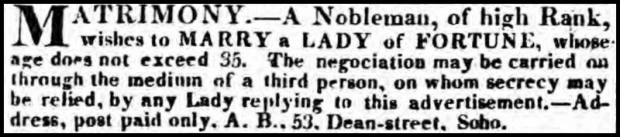
\includegraphics[width=0.45\textwidth]{figures/Introduction/morning-post-june-25-1823.png}\label{fig:img1_a}}\hfill
    \subfigure[]{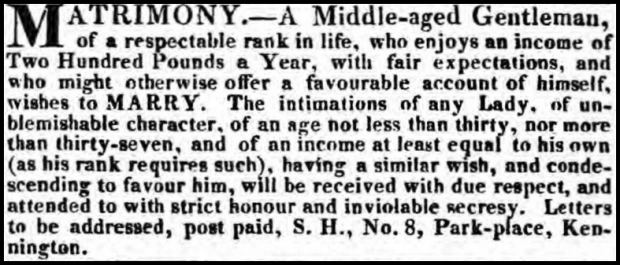
\includegraphics[width=0.45\textwidth]{figures/Introduction/morning-post-december-19-1822.png}\label{fig:img1_b}} 
    \caption{Matrimonial Advertisements in London’s \textit{Morning Post} in the 19th Century}
    \label{fig:img1}
\end{figure}

As the 19th century progressed, the popularity of matrimonial advertisements continued to grow, leading to the emergence of matrimonial specialty magazines like the Matrimonial News and the Matrimonial Intelligencer. These publications were dedicated solely to marriage and complemented the abundance of matrimonial ads found in newspapers, including those targeting specific religious audiences. Religion often played a significant role in these advertisements, highlighting the importance of shared faith in potential matches. Matrimonial ads provided an economical and accessible way for individuals who lacked family, friends, or financial resources to make meaningful connections and seek spouses.\cite{noauthor_alternative_2016}. Figure \ref{fig:img1} shows some of the examples advertisements posted in the newspapers during the 19th century. 

The concept of dating began to take shape at the turn of the 20th century, moving away from the more formal and structured courtship practices of earlier times. Dating became more informal and less focused on immediate marriage, reflecting broader social changes and evolving attitudes toward romantic relationships. This period saw the emergence of "dating" as a distinct phase of a relationship, where couples would spend time together outside the home without the immediate expectation of marriage. This shift was part of a larger cultural change that placed greater emphasis on personal choice and romantic love over social and economic considerations in mate selection. \cite{markarian_how_2017}. In the early 20th century, "Mechanical Matchmaking" emerged, with a notable example being the attempt by Hugo Gernsback, the publisher of Science and Invention magazine, to apply scientific methods to matchmaking. In April 1924, Gernsback proposed four "scientific" tests to determine the likelihood of marital success, including physical attraction tests, sympathy tests, body odor tests, and nervous disorder tests. These methods aimed to quantify and predict the success of marriages, illustrating an early fascination with applying technology and science to personal relationships, much like today's online dating algorithms.\cite{magazine_mechanical_nodate}. In the 1950s, a Newark based, matchmaking service called Introduction, used data as a foundation of their matchmaking services and charged a fee for ‘personalized’ recommendations of suitable matches based on qualifications and social status and subsequent sharing of contact information. \cite{newark_introduction_nodate}

One landmark development in the fusion of technology and dating was Operation Match, which emerged from Harvard University in 1965. Developed by undergraduate students Jeff Tarr and Vaughan Morrill, along with Doug Ginsberg and David Crump, Operation Match was conceived as an innovative solution to the challenges of dating life on campus. Utilizing an IBM 1401 computer, the service employed a sophisticated algorithm to match individuals based on their responses to a comprehensive questionnaire covering personal preferences and interests.\cite{noauthor_operation_1965}  Participants of Operation Match filled out lengthy questionnaires, which they submitted with \$3, and a program on an IBM 1401 computer would match questionnaires to similar responses.\cite{valley_new_2015}  The questionnaires were then transferred to punched cards and processed on an IBM 7090 computer and users received an IBM 1401 print out in the mail a week later, listing the names and contact information of potentially suitable matches. The increased sophistication provided by the IBM 1400 series propelled computer matchmaking into the public shhere as commercial matchmaking servics adopted advanced means to help singles find suitable dates. This increase in popularity of preferenced based match making combined with sexual revolution of the 1960s and 1970s, because of the introduction of oral contraceptives in the 1960s, the rising visibility of the LGBTQ+ community along with the second-wave of feminist movement,\cite{book:1309549} brought upon a drastic change in the attitudes of the people towards dating and relationships. From a culture that only endorsed serious relationships and marriage with the flexibility to choose a sociall equivalent partner, the society started to accept casual dating and hookups. The culture encouraged an individual to explore for their options both sexually and romantically, with multiple partners without any restrictions based on social strata and also having no end goal of marriage. The emergence of modern dating practices offered unprecedented opportunities for social mobility and the exploration of sexuality, albeit within the constraints of the era. This development represented a significant departure from traditional expectations, which often confined individuals to relationships with partners from specific, socially sanctioned groups. Women, in particular, experienced a notable expansion of autonomy through the relaxation of socio-cultural restrictions\cite{book:1309549}. This newfound freedom enabled them to date, form romantic attachments, and partake in sexual relationships with greater agency. 

\begin{figure}[t!]
 \centering
 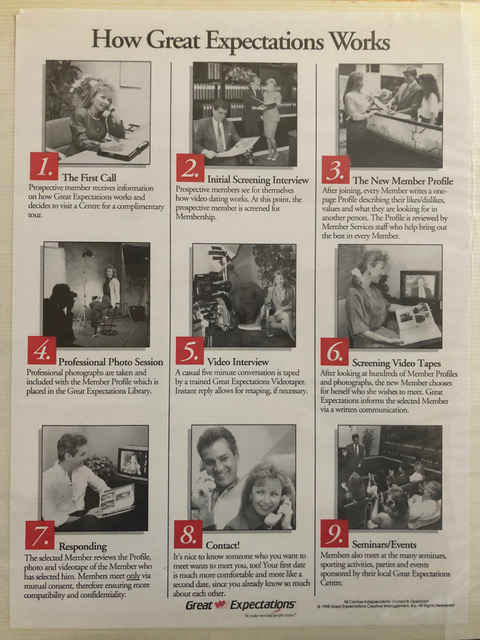
\includegraphics[scale=0.6]{figures/Introduction/GE2.png}
 \caption{A flyer explaining how Great Expectations works}
 \label{fig:img2}
\end{figure}

In the 1980s, post the rise of computer matchmaking, video matchmaking started to emerge. Video (or VHS) dating brought along with it a new way to meet potential partners, with added dimension of being able to hear and see the person before meeting them in person. The first known video dating service was started by Jeffrey Ullman in 1983, called the Great Expectations.\cite{waters_how_2021}. In video matchmaking, participants were asked a series of personal and motivational questions, such as their work ethic, triggers for anger, sources of motivation, and qualities they sought in a partner. After these interviews were recorded, the videotapes were cataloged in a video dating library. Members could browse through this collection, aided by a one-page profile attached to each video that included key details like height, location, and occupation, allowing them to screen potential matches before watching a tape. Figure \ref{fig:img2}, shows a flyer explaining how Great Expectations works. Hearing and Viewing the partners before selecting them was a significant advantage, because as Ullman said ``it showcased a more honest version of a person". \cite{waters_how_2021} This method brought out some of the marvellous personalities of people that would not show up just based on a written questionnaire as was the case in the previous approaches. But the hype of video dating dwindled in the early 1990s because of how cumbersome the process was. It did not bring out a massive change in the dating culture, but it did pave the way for the design of modern dating applications. 

The terminology "matchmaking" is purposefully employed in the preceding sections to delineate pre-Match.com "dating" mechanisms, as these early technologies primarily served the function of facilitating introductions between two parties deemed compatible on a multitude of criteria, ranging from social status to individual predilections and shared ideologies. Prior to the digital revolution instigated by Match.com, "dating" technologies were constrained to the matchmaking domain, enabling initial introductions without encompassing the subsequent phase of dating, which is crucial for assessing compatibility through real-world interactions. The advent of the internet, and specifically Match.com, heralded a paradigm shift by amalgamating matchmaking and dating within a unified online platform. Match.com was instrumental in revolutionizing the dating industry by accelerating the matchmaking process and introducing communication features like chat boxes, thereby allowing matches to engage in preliminary interactions ('date') prior to arranging face-to-face encounters.\cite{noauthor_dating_nodate} This platform introduced the concept of a 'dating profile', encouraging users to provide personal insights alongside photographs, thereby streamlining the process of discovering and interacting with potential matches within a singular service. Contrasting with prior methodologies, which necessitated intermediary involvement and were characterized by significant delays, online dating platforms provided immediate access to an expansive pool of potential matches, along with the autonomy to evaluate compatibility through direct communication, thus enhancing the process's transparency, dynamism, and efficiency.

The evolution of dating technologies further advanced with the development of mobile dating applications, such as Tinder and Bumble, transforming the dating experience into a mobile-centric endeavor. These applications, extensively discussed in the second chapter, innovated user interaction through the implementation of the 'swipe' mechanism and a pronounced focus on visual self-presentation\cite{noauthor_dating_nodate, marcus2016swipe} Notably, such applications significantly contributed to normalizing the sexual exploration or 'hook-up' culture, making it openly accessible and socially acceptable across various demographics\cite{noauthor_dating_nodate, marcus2016swipe}. Tinder, for instance, played a pivotal role in normalizing explicit expressions of sexual intentions by incorporating features that allow users to specify their looking-for preferences, such as casual encounters or long-term relationships, directly on their profiles. Employing sophisticated algorithms and engaging chat functionalities, including emojis, GIFs, and memes, these applications further refined the match screening process, enabling users to make more informed decisions regarding the viability of face-to-face meetings.

This transition from traditional matchmaking services to comprehensive online dating platforms has significantly broadened the interaction spectrum, empowering users to exercise greater selectivity in their dating pursuits. By facilitating a virtual screening process, these digital mediums have not only conserved time and effort but have also expanded the horizons for establishing and nurturing romantic connections in the contemporary era, underscoring a profound shift in the landscape of dating technologies.


\subsection{The Indian Context}
The evolution of dating and matrimony technologies in India has been influenced by the country's unique socio-cultural landscape, characterized by a rich tapestry of traditions, values, and familial structures. It is evident from the previous section that the Western dating culture has undergone significant transformations over the centuries, transitioning from arranged marriages to companionate marriages and subsequently embracing casual dating and hook-up culture. In contrast, to the technologies in the west, dating technology were modified to server as matrimonial services because of the social unacceptability of any form of Dating in the Indian society, until the 2000s \cite{doshi_date_2016, noauthor_modern_2017, sharma_towards_2019}. 

Traditionally, relationships and marriages in India were orchestrated through family networks or arranged by parents, emphasizing communal ties over individual choice. However, the late 20th and early 21st centuries marked a significant transition, driven by technological advancements and a growing emphasis on individual autonomy in choosing romantic partners. Personal advertisements were predominantly utilized to identify appropriate marital alliances, and the inception of Shaadi.com, shortly after the launch of Match.com, mirrored this utility, albeit within the matrimonial context of Indian society. In this cultural milieu, the responsibility of selecting suitable marital candidates traditionally rested with the parents, given the substantial emphasis placed on variables such as caste, religious affiliation, and upbringing. These factors not only held, but continue to hold, considerable importance, with parents extensively relying on their expansive social networks to discover apt matches for their offspring \cite{sharma_towards_2019, seth_online_2008}. Matrimonial services remained largely unchanged, focusing predominantly on matchmaking, as the prerogative to sift through recommended matches was vested in the parents of the concerned individuals, thereby obviating the necessity for incorporating 'dating experiences' to vet multiple prospective partners \cite{titzmann_changing_2013}. The paramount decision-making authority resided with the parents, thus constraining opportunities for dating or romantic exploration—until the widespread adoption of mobile phones in the early 2000s. Mobile telephony and the internet introduced novel avenues for discreet dating, facilitating the quest for partners beyond the traditional constraints of caste and religious affiliations. It is pertinent to highlight that, at this juncture, the Indian dating paradigm mirrored Western practices of the early twentieth century, predominantly aimed at culminating in 'love marriages.'

Liberalization of the Indian economy also played a pivotal role in the introduction of dating applications in India. Liberalization brought upon a transformation in the image of the traditional image of the middle-calss wife India. Traditionally, the middle-class wife in India was emblematic of virtues such as modesty, submissiveness, and a strong adherence to family values, often confined within the domestic sphere and her roles as a caregiver and moral guardian of the family. This portrayal underscored the gender norms and cultural expectations deeply ingrained in the patriarchal fabric of Indian society, where a woman's identity was largely defined through her relationships with men as a daughter, wife, and mother \cite{Dell_2005}.

The onset of economic liberalization introduced a wave of change, marking a pivotal shift in the socio-economic landscape of India. This period was characterized by the opening up of the Indian economy to global markets, an influx of foreign investment, and the adoption of neoliberal policies. Concurrently, this economic shift brought about a significant social transformation, particularly in the roles and perceptions of women in Indian society. The liberalization era ushered in increased educational and employment opportunities for women, challenging the traditional confines of their roles within the household and promoting a narrative of economic empowerment and independence for women. This marked departure from traditional roles was not merely an economic transition but also a cultural shift, fostering a reevaluation of gender dynamics and the emergence of new models of femininity and partnership inspired by global media and the internet \cite{Forbes_2020}.

The increased visibility of women in the workforce and their active participation in public and political spheres echoed the growing feminist movements in India. These movements advocated for gender equality, challenging the patriarchal status quo and pushing for legal and social reforms to address gender discrimination, marital rights, and issues of domestic violence. The discourse around marriage and relationships also evolved, reflecting a gradual shift towards mutual respect, companionship, and shared responsibilities between partners. The liberalization era, therefore, not only transformed the economic landscape but also significantly impacted the social fabric of India, reshaping traditional notions of womanhood and partnership \cite{statista_internet_users_2050}.

In the realm of dating and relationships, the impact of liberalization was further evidenced by the growing acceptance of love marriages, inter-caste and inter-religious unions, and the concept of dating itself—practices once considered taboo. 

The landscape of Indian dating culture witnessed a profound transformation in 2011 with Tinder's entry into the Indian market. Marketed primarily as a 'hook-up' application, Tinder swiftly gained traction among the youth, thereby democratizing dating and, notably, casual romantic encounters. The prevailing narratives suggest a gradual shift from a staunchly arranged marriage-oriented society towards a more open acceptance of 'dating' among the younger demographic. This cultural evolution is fostering the emergence of varied dating practices, spanning from serious relationships to casual dating and hook-ups. The locus of choosing a partner is increasingly transitioning from parents to the individuals themselves, buoyed by the rising popularity of online dating platforms such as OkCupid and Tinder. This paradigm shift towards individual agency in partner selection is a relatively recent development, with online dating gaining the quickest acceptance among college students and young professionals \cite{doshi_date_2016}.

The introduction of dating applications such as Tinder, OkCupid, and Bumble marked a significant cultural shift, offering an alternative to the traditional pathways to marriage. These platforms provided a space for individuals to explore romantic relationships without the immediate objective of marriage, thereby allowing for greater personal autonomy in matters of love and partnership \cite{Das_2019}. his shift is reflective of a broader global trend where individual choice and compatibility are increasingly valued over traditional matchmaking criteria.

The Chief Marketing Officer of OkCupid highlighted the unique nature of the Indian market, noting that a generation of young Indian women is redefining relationship norms by asserting their right to choose their partners. This sentiment encapsulates the transformative impact of dating apps, empowering individuals, especially women, to exercise greater control over their romantic lives "What makes India different is that we have a generation of young women who are changing things by saying, ‘I want to decide who I’m with’" \cite{Forbes_2020}.

In response to the cultural and societal nuances of the Indian context, homegrown applications like TrulyMadly and Aisle have emerged, blending traditional values with modern dating practices. These platforms are designed to cater to the Indian audience's preferences, striking a balance between casual dating and the pursuit of long-term partnerships. By incorporating cultural sensibilities into their algorithms and features, these apps offer a "middle ground" that respects the societal norms and expectations prevalent in Indian society \cite{Forbes_2020}. Bumble, in particular, has made a notable impact by emphasizing women's empowerment through its unique feature that allows only women to initiate conversations.\cite{noauthor_bumble_nodate} This approach not only challenges traditional gender dynamics but also promotes a safer and more respectful online dating environment for women, aligning with broader movements for gender equality and women's rights in India. The rise of dating applications in India is emblematic of the country's ongoing negotiation between tradition and modernity. As India continues to evolve socially and economically, these platforms reflect and facilitate changing attitudes towards relationships, marriage, and personal autonomy. Moreover, the success and adaptation of these platforms in India underscore the globalized nature of technological and cultural exchange, where Western innovations are localized to fit the specific needs and contexts of different societies.

The embrace of Bumble's features by women in India marks a notable shift in the country's dating culture. Women making the first move over 15 million times and sending twice the number of messages compared to the global average highlights a significant change in gender dynamics within the dating scene. This statistic not only signifies women's acceptance of the platform but also their active engagement in shaping their romantic interactions, which is a departure from the traditionally passive role attributed to women in the courtship process in India (Hindustan Times, 2020).

Moreover, the fact that 32\% of women users in India use more than one mode on Bumble suggests that the app is being used not just for dating but also for forming broader social connections. This indicates a broader application of the app's features, possibly extending to networking and friendship, reflecting a versatile use of technology to fulfill various social needs \cite{HindustanTimes_2020}. Further emphasizing the influence of contemporary culture on dating preferences, a recent Bumble report highlights how social media, music, food, literature, and content consumption are shaping Gen Z's dating ideals in India. These factors are indicative of a more globalized approach to dating where personal interests and cultural consumption significantly influence romantic connections \cite{Chronicle_2023}.

Additionally, changes in dating preferences show a trend towards virtual dating, with predictions that 40\% of single Indians will favor this mode of interaction. This reflects a growing comfort with digital interactions and an appreciation for the importance of education, career choices, and compatibility as bases for forming relationships, beyond just physical or geographical proximity \cite{MediaInfoline_2021}. The integration of technology into personal relationships is not unique to India. Globally, dating apps have reshaped social interactions. For instance, in the United States, Tinder and similar apps have significantly influenced dating norms, with studies indicating that online interactions have become a primary way young people connect romantically and socially. These platforms provide a space where users can express themselves in ways that may not be possible in their immediate physical environments, thus expanding their social horizons \cite{Smith_2016}.

The introduction of Bumble in India has marked a significant development in the visibility and social acceptance of LGBTQIA+ identities within the country. The platform’s proactive stance on inclusivity and safety has played a crucial role in not just providing a dating service but also advocating for the rights and recognition of LGBTQIA+ individuals in a society where their acceptance remains inconsistent. The decriminalization of gay sex by the Supreme Court of India in 2018 \cite{Johar} was a landmark moment, legally abolishing Section 377, a colonial-era law that criminalized homosexual acts. However, legal acceptance does not automatically translate into social acceptance, and the LGBTQIA+ community continues to face various forms of discrimination and stigma. In this context, platforms like Bumble serve as important spaces for safe social interaction and self-expression for LGBTQIA+ individuals.

Bumble has introduced several features aimed specifically at enhancing the safety and inclusivity of its platform for LGBTQIA+ users:

\begin{itemize}
    \item \textbf{Guides for Queer Dating:} Bumble provides tailored guides that offer advice and support for queer dating, addressing the unique challenges faced by LGBTQIA+ individuals in navigating the dating world. \cite{Bumble}
    \item \textbf{Incognito Mode:} This feature allows users to maintain privacy and control over who sees their profile, giving LGBTQIA+ users the discretion they may need in a conservative society. \cite{Bumble_incognito}
    \item \textbf{Private Detector:} Bumble’s private detector automatically blurs lewd images to protect users from unsolicited explicit images, enhancing the safety of interactions. \cite{Bumble_private_detector}a
    \item \textbf{Photo Verification:} This feature helps to ensure that profiles are genuine, reducing the risk of catfishing and improving trust and safety on the platform. \cite{Bumble_photo_verification}
    \item \textbf{Pronoun Selection:} By allowing users to select and display their pronouns, Bumble fosters an environment of respect and recognition for gender identity, which is particularly important for transgender and non-binary individuals. \cite{Bumble_pronoun_feature}
\end{itemize}

Bumble’s efforts extend beyond individual safety to influence broader social perceptions and norms regarding LGBTQIA+ identities. By normalizing the inclusion of diverse sexual orientations and gender identities in its platform, Bumble challenges societal prejudices and promotes greater visibility and acceptance of the LGBTQIA+ community. This visibility is crucial in changing public attitudes and encouraging more open discussions about LGBTQIA+ issues in India. Research on the impact of dating apps on LGBTQIA+ communities indicates that such platforms can significantly affect users' lives by providing spaces for identity exploration and community building that are often unavailable in other areas of their lives. Studies suggest that dating apps can help lower barriers to social interaction and empower users by allowing them to seek out connections on their own terms \cite{Blackwell_2015}. Moreover, the role of technology in shaping cultural and social dynamics is increasingly recognized, with scholars arguing that digital platforms can play a transformative role in challenging traditional norms and advocating for marginalized communities \cite{Publishers_Distributors4753/23_Road_Delhi}.

\section{Fairness in AI systems}
The widespread adoption of recommendation algorithms across digital platforms, ranging from online shopping to social media, has sparked a growing awareness of their capacity to perpetuate social injustices. These algorithms are fundamental in shaping user experiences by predicting and influencing behavior through the processing of vast datasets. However, despite their utility, they frequently mirror and even magnify existing societal biases, embedded unintentionally within the data they analyze. This issue arises from algorithms learning from real-world data that reflects historical inequalities or prevalent stereotypes, leading to decisions that systematically disadvantage certain groups.

The inadvertent reinforcement of biases by algorithms not only affects the fairness of automated decisions but also raises ethical concerns about the integrity of AI systems in various applications. As these systems become more integral to everyday life, the urgency for addressing these biases grows, necessitating a careful examination of how algorithms interact with societal norms and structures. Researchers have argued for the development of methods to detect and mitigate biases in AI systems as a critical step towards ensuring they promote equity and fairness. The challenge lies in the inherent complexity of AI models and the subtlety with which biases can be integrated into algorithmic decisions, often masked by the technical opacity of these systems.

Significant scholarly attention has been directed towards understanding the scope and impact of algorithmic bias. Studies have consistently highlighted the need for transparency in AI processes and the implementation of robust fairness metrics to evaluate and rectify biases. The push towards ethical AI involves a multidisciplinary approach, incorporating insights from computer science, social sciences, and legal studies to create AI systems that are not only effective but also equitable and just.

Therefore, addressing these challenges is not merely a technical task but a societal imperative, requiring concerted efforts from developers, regulators, and users alike. Ensuring the fairness of AI systems is fundamental to harnessing the full potential of this technology in a way that benefits all sections of society equitably, fostering trust and wider acceptance of AI applications across various domains.

In recent years, numerous cases have highlighted the inherent risks of discrimination and biases embedded in AI systems, particularly those used in recommendation engines and automated decision-making. These issues not only raise ethical concerns but also underscore the need for more robust frameworks to ensure fairness in AI deployments.

\subsection{Racial Bias in Judicial Algorithms}
One of the most notable instances of AI bias is seen in the COMPAS algorithm, used in the criminal justice system in the United States. This algorithm was found to misclassify black defendants as having a higher risk of reoffending compared to their white counterparts, leading to unfairly harsher sentencing and bail decisions. This case underscored the racial biases that can be perpetuated by automated systems, raising alarms about the fairness and impartiality of using AI in legal contexts \cite{Mattu}.

\subsection{Gender Bias in Job Advertisements}
Another significant example is the gender bias in job advertising on platforms like Facebook, where algorithms were found to display ads for high-paying job opportunities more frequently to men than to women. This was not the result of explicit programmer intent but rather the outcome of the algorithm learning from existing societal biases, indicating that without careful oversight, AI systems can reinforce and perpetuate existing inequalities \cite{Lambrecht_Tucker_2019}.

XING, a professional networking and job recruitment platform similar to LinkedIn, has also faced scrutiny for biases in its job recommendation algorithms. A notable instance of this was highlighted in a study that found XING's algorithms recommended more underqualified men for certain jobs than qualified women. This disparity suggests the presence of gender bias within the algorithm's decision-making processes.

The study indicated that such biases could stem from the training data used to develop these algorithms. If the historical data on which these systems are trained contain gender imbalances—for instance, more men being hired for certain types of jobs than women—algorithms may inadvertently learn to perpetuate these patterns. This results in a feedback loop where men continue to be favored over equally or more qualified women, reinforcing gender inequality in professional settings.\cite{Lahoti_Gummadi_Weikum_2019}

\subsection{Bias in Mortgage Applications}
AI systems have also been implicated in biases affecting mortgage approval processes. Research has shown that automated algorithms used by financial institutions to determine eligibility for loans were less likely to approve loans for applicants from minority backgrounds compared to similar white applicants. This kind of financial bias has significant long-term impacts on wealth accumulation and equality in access to housing \cite{Bartlett_Morse_Stanton_Wallace_2022}

\subsection{Bias in Facial Recognition Technologies}
Facial recognition technologies, widely used in surveillance and security applications, have been criticized for their higher rates of misidentification among people of color, particularly black individuals, and women. This not only raises privacy concerns but also poses a risk of wrongful accusations in law enforcement and security settings. Studies have shown that these biases are due to the underrepresentation of these groups in the training datasets used to develop these technologies \cite{Buolamwini_Gebru_2018}

\subsection{Ethical Concerns in Healthcare Algorithms}
In healthcare, algorithms designed to predict patient health outcomes and allocate healthcare resources have shown biases against certain demographic groups. For example, an algorithm widely used in U.S. hospitals was found to be biased against black patients in its predictions of healthcare needs, resulting in less healthcare resources being allocated to black patients compared to white patients with similar conditions. \cite{Obermeyer_Powers_Vogeli_Mullainathan_2019}

%--------------------------------------------------------

\chapter{Methodology}
\label{ch:methodology}
This chapter delineates the methodology adopted in this thesis to explore gender disparities in Bumble’s match recommendations. The research design incorporates qualitative, quantitative, and mixed methods to furnish a comprehensive analysis of algorithmic biases \cite{Kalra_Gupta_Varghese_Rangaswamy_2023}. This chapter explicates the procedural framework utilized for participant selection, ensuring a representation that mirrors the diverse demographic of Bumble users, crucial for the validity of the findings \cite{Mislove_Viswanath_Gummadi_Druschel_2010}.

Data were collected through a combination of surveys, structured interviews, and meticulous profile analysis, with each method carefully selected to address specific research questions \cite{Kalra_Gupta_Varghese_Rangaswamy_2023}. This multimodal approach enables a thorough investigation into the algorithmic processes and their implications on user experience and bias reproduction. Ethical considerations are paramount, guiding all data collection activities to ensure compliance with research ethics standards and participant privacy \cite{Elovici_Fire_Herzberg_Shulman_2014}.

The data analysis procedures employed are detailed subsequently, highlighting the analytical techniques and statistical methods used to dissect the complex interplay between user behavior and algorithmic recommendations. This robust analytical approach allows for nuanced insights into how gender biases may manifest in digital matchmaking environments \cite{Raghavan_Barocas_Kleinberg_Levy_2019}.

The chapter concludes with a discussion on the limitations of the research design and potential biases that may influence the findings. Strategies to mitigate these limitations are proposed, emphasizing the need for transparency and reflexivity in algorithmic research. The chapter sets the stage for the subsequent chapters, which delve into the empirical findings and theoretical implications of the study.

\section{Research Design}
\subsection{Selection of Research Methodology}
This study employs a mixed-methods approach, integrating both qualitative and quantitative research methodologies to provide a robust analysis of the algorithmic biases present in Bumble's matchmaking system. The rationale for adopting a mixed-methods approach is to capitalize on the strengths of both qualitative and quantitative research in uncovering nuanced insights into the algorithmic processes and their effects on different genders. Mixed methods allow for a comprehensive understanding of both the measurable trends through quantitative analysis and the subjective experiences through qualitative insights \cite{Kalra_Gupta_Varghese_Rangaswamy_2023}. 

\subsection{Quantitative Research Component}
The quantitative aspect of this research primarily revolves around the use of surveys and profile analysis. This component is crucial for obtaining measurable data on user interactions and algorithmic output, which can be statistically analyzed to detect patterns of bias or discrepancies in match recommendations across different gender identities.

\begin{itemize}
    \item \textbf{Surveys:} Structured surveys were administered to a diverse group of Bumble users to gather data on user satisfaction and perceived fairness in match recommendations. The surveys included both closed and open-ended questions, allowing for the collection of both quantitative data and qualitative feedback.
    \item \textbf{Profile Analysis:} An analytical review of user profiles was conducted to quantitatively assess how the algorithm categorizes and prioritizes user profiles. This involved collecting data on factors such as frequency of matches, user preferences, and the diversity of profile recommendations. 
\end{itemize}

\subsection{Qualitative Research Component}
The qualitative component focuses on interviews and thematic analysis, providing deeper insights into the personal experiences of users and their perceptions of algorithmic bias.

\begin{itemize}
    \item \textbf{Interviews:} Semi-structured interviews were conducted with selected Bumble users who have experienced varying levels of interaction and success on the platform. These interviews helped to uncover personal narratives that illustrate the impact of algorithmic decisions on real-world social interactions and relationships.
    \item \textbf{Thematic Analysis:} Responses from interviews and open-ended survey questions were subjected to thematic analysis to identify common themes and patterns that may not be immediately evident through quantitative methods alone.
\end{itemize}

\subsection{Integration of Research Components}
The integration of quantitative and qualitative components in this mixed-methods design facilitates a more comprehensive understanding of both the statistical and humanistic aspects of algorithmic bias in dating apps. This approach not only provides a broad statistical overview of user experiences but also delves deeply into individual stories and perspectives, enriching the interpretation of data with personal contexts and nuanced insights.


This mixed-methods research design is meticulously crafted to explore the intricate dynamics of algorithmic matchmaking in a popular online dating platform. By combining quantitative data analysis with qualitative inquiries, the study aims to provide a holistic view of the algorithmic biases that potentially affect gender disparities in match recommendations. The methodological rigor and interdisciplinary approach ensure that the findings contribute valuable insights into the ongoing discussions about fairness and inclusivity in digital environments.

\section{Participant Selection and Demographics}
In this study, a purposive sampling technique was employed to select participants who were active or past users of Bumble, ensuring a focus on individuals directly impacted by the matchmaking algorithms of the platform. This method of sampling is critical for qualitative research where the need for specific types of information arises, and where the researcher seeks to understand common themes across a specific group of people.

\subsection{Criteria for Participant Selection}
Participants were selected based on several criteria:

\begin{itemize}
    \item \textbf{Age:} All participants were within the age group of 18-24 years, aligning with Bumble’s primary user demographic in urban areas like Mumbai, where the study was focused.
    \item \textbf{Usage:} Both current and past users of Bumble were included to gain perspectives from active users and those who may have discontinued use due to dissatisfaction or other reasons.
    \item \textbf{Gender Identity:} The study targeted a balanced representation across different genders, including cisgender men and women, as well as non-binary individuals. This was crucial to explore the differential impacts of algorithmic biases across these groups.
\end{itemize}

\subsection{Demographic Breakdown}
The participant pool for the profile analysis consisted of:
\begin{itemize}
    \item Two self-idenitfied men
    \item Two self-idenitfied women
    \item One self-idenitfied non-binary person
\end{itemize}

The participant pool for the interviews included:
\begin{itemize}
    \item Three self-identified cis-men
    \item Two self-identified bisexual-men
    \item Three self-idenitfied cis-women
    \item One self-idenitfied bisexual-woman
    \item One self-idenitfied bisexual non-binary person
\end{itemize}
This demographic mix was instrumental in exploring the nuances of how gender impacts user experience on Bumble, particularly in the context of algorithmic matchmaking.

Mumbai was selected as the primary location for participant recruitment. Mumbai was chosen due to its high urban population and technological savviness, factors which contribute to a diverse user base with varied dating preferences. This diversity is essential for examining the complex dynamics of Bumble's matchmaking algorithm and its adaptability to different user profiles. Mumbai's cultural richness and demographic diversity provide a unique context for exploring how cultural and societal norms influence dating behaviors and attitudes towards the LGBTQIA+ community. These factors are critical in understanding how users interact with the app and each other, potentially affecting the algorithm's function and effectiveness in making match recommendations. The choice of Mumbai impacts the study by introducing specific cultural and demographic variables that may influence user behavior and algorithmic responses. These include varying levels of social acceptance, stigma towards different gender identities, and the overall openness of the community to online dating. Such factors are anticipated to play a significant role in shaping the data collected, particularly concerning how different genders experience the platform.

\subsection{Ethical Consideration}
In recruiting participants, ethical considerations were strictly adhered to, with all participants providing informed consent. The research design included protocols to protect participant anonymity and confidentiality, which is particularly important given the sensitive nature of data related to personal relationships and dating behaviors. Ethical guidelines from the International Institute of Information Technology, Hyderabad, were followed to ensure the study’s integrity and the welfare of all participants \cite{Kalra_Gupta_Varghese_Rangaswamy_2023}.

\subsection{Additional Considerations}
To deepen the understanding of the dataset and enhance the robustness of the study, it would also be beneficial to consider:

\begin{itemize}
    \item \textbf{Socioeconommic Status:} Future research could include participants from varied socioeconomic backgrounds to examine if and how socioeconomic factors influence user experiences and interactions with the Bumble algorithm.
    \item \textbf{Demographic Status:} While this study focused on Mumbai, expanding the research to include other cities or rural areas could provide insights into regional variations in algorithmic impact, reflecting broader demographic trends and preferences.
\end{itemize}


The selection of participants and the demographic characteristics are pivotal in research as they directly influence the reliability and applicability of the findings. A well-rounded demographic profile supports the generalization of the study results to a broader population and ensures that the conclusions drawn are reflective of diverse user experiences, thereby enhancing the study’s credibility and relevance in discussions on algorithmic fairness in social platforms.

This approach not only fulfills the research’s methodological needs but also aligns with broader ethical and scholarly standards, ensuring that the study’s outcomes can effectively contribute to ongoing debates and future policymaking in the realm of digital dating and algorithmic mediation.

\section{Data Collection Methods}
This study utilized a comprehensive multi-method approach to collect data, employing surveys, interviews, and profile analysis to capture both quantitative and qualitative insights into user experiences and algorithmic performance on Bumble \cite{Kalra_Gupta_Varghese_Rangaswamy_2023}. Each method was chosen to complement and enhance the insights gained from the others, ensuring a robust analysis of the algorithms’ impact across different demographic groups.

\subsection{Surveys}
Structured surveys were administered to a diverse group of Bumble users to quantitatively assess their satisfaction and perceived fairness in match recommendations. These surveys included a mix of scaled responses and open-ended questions to facilitate quantitative analysis of user satisfaction and qualitative insights into user perceptions and experiences.

\begin{itemize}
    \item \textbf{Design and Distribution:} The surveys were designed to be comprehensive yet concise, ensuring a high completion rate. They were distributed electronically via email and social media platforms, targeting users from the demographic groups identified in the participant selection phase. 
    \item \textbf{Content:}  Questions focused on user satisfaction with the matches received, perceived biases in the recommendation system, and personal impact of these biases. This included asking participants to rate their satisfaction on a Likert scale and provide narrative descriptions of their experiences.
\end{itemize}

\subsection{Profile Analysis}
Profile analysis in this study was meticulously designed to quantitatively examine the operation of Bumble’s matchmaking algorithm, focusing particularly on the algorithm's handling of diverse gender identities. This analysis aimed to uncover potential biases and operational patterns by observing the profiles shown to users and the interactions these profiles elicited. The decision to focus particularly on non-binary genders stemmed from a gap identified in existing research, which often centers around the binary genders of male and female. Non-binary individuals frequently face unique challenges and biases on dating platforms, which can be overshadowed in broader algorithmic studies. By concentrating on this demographic, the study sought to illuminate the specific ways in which non-binary profiles are treated differently by the algorithm, providing insights into inclusivity and fairness of the platform. Bumble allows users to select from an extensive list of gender identities, which includes but is not limited to Man, Woman, Non-Binary, Transgender Man, Transgender Woman, Genderfluid, Genderqueer, Gender Non-conforming, and Two-Spirit. We made a conscious choice of non-binary to be less specific about gender preference and also to adhere to the conventions of  Bumble, which showcases the major genders as man, woman and non-Binary. 

\begin{itemize}
    \item \textbf{Data Collection:} Data was captured on various attributes of the profiles recommended to users, including age, gender, location, and interests.
    \item \textbf{Analysis:} The analysis focused on understanding the correlations between user preferences (as indicated in their profiles and swipe behavior) and the characteristics of the profiles recommended to them. Special attention was given to discrepancies in recommendations across different genders.
\end{itemize}

The data displayed on each user profile is selected voluntarily by the individual when setting up their account on Bumble. Users have the discretion to include or omit various details, such as age, occupation, and location, among others. While not mandatory, filling out these profile attributes is encouraged by Bumble, as the platform suggests that a more complete profile enhances the algorithm's ability to match users with potential suitors who are likely to be more compatible. This feature underlines the balance between user privacy and the effectiveness of the matchmaking process, suggesting that richer profile information can lead to more meaningful connections.

To supplement the observational data from surveys and profiles, an experimental design could also be employed where user interactions are simulated under controlled conditions to observe the outcomes of specific changes in the algorithm. This method would allow researchers to isolate specific factors and directly measure the algorithm’s responsiveness to controlled variations in user behavior and profile settings.

With the latest updates to Bumble's mobile application, the methodology employed in the profile analysis requires an update to account for these changes. The previous analysis conducted on the web version of Bumble required non-binary users to select whether they wanted their profiles to appear in searches for men or women. However, the mobile application has now eliminated this requirement, allowing non-binary users to be displayed without having to categorize themselves within the binary gender options. This significant platform update necessitates a reevaluation of the research methodology and a comparative analysis to determine if these application changes affect the user experience and algorithmic output for non-binary users.

\subsection{Interviews}
Interviews in this study were designed to gather in-depth qualitative data from Bumble users, providing a deeper understanding of individual experiences and perceptions regarding the app's matchmaking algorithm. The semi-structured nature of these interviews allowed for flexibility, letting participants freely express their thoughts while still guiding the conversation to cover specific topics of interest essential to the research questions. Participants for the interviews were selected based on their responses to the initial survey. Those who indicated particularly insightful or unique experiences with Bumble—such as perceived biases or significant impacts on their dating life—were chosen to provide a richer, more detailed account of their interactions with the platform.

The interview process was as follows:
\begin{itemize}
    \item \textbf{Preparation:} Ahead of the interviews, a guide was prepared with open-ended questions to explore themes like user satisfaction, perceived fairness, and personal stories of match interactions. Example questions included:
    \begin{itemize}
        \item "Can you describe any patterns you've noticed in the matches you receive?"
        \item "How do these patterns align with your expectations and preferences?"
        \item "Have you ever felt that your profile was treated differently compared to others? Please elaborate."
    \end{itemize}
    \item \textbf{Conducting Interviews:} Interviews were conducted via video calls to accommodate the participants' geographical diversity and recorded with their permission for accuracy in data collection. Each session lasted approximately 30-45 minutes.
    \item \textbf{Data Handling:} All interviews were transcribed verbatim, and identifying information was anonymized to maintain confidentiality. The transcripts were then analyzed using thematic analysis to identify common themes and significant outliers in user experiences.
\end{itemize}

\section{Ethical Concerns}
In this section, we will first attempt to identify the potential ethical concerns that can arise while conducting this experiment. The ethical issues that are relevant to us are the ones that are morally wrong things or can any problematic outcomes that can be a result of this experiment. After identifying, we will either attempt to justify how an ethical concern can be ignored or explain what steps we are taking to counter these ethical concerns. The potential ethical issues that we see are as follows:
\begin{itemize}
	\item Informed consent: It is essential to ensure that all participants fully understand the nature and purpose of the study and any potential risks or benefits before they agree to participate. This means that the researchers must provide clear and comprehensive information about the study and ensure that participants can ask questions and raise concerns.
	\item Confidentiality: The researchers must ensure that the personal information of the participants is kept confidential and secure. This includes any data collected about the profiles recommended to them and any information about their profiles and interactions on the Bumble platform.
	\item Deception: The use of fake profiles in this study may be seen as a form of deception, as the participants' actual gender will not be disclosed on one of their profiles. This could be unethical, as it may cause some participants to feel misled or manipulated. To mitigate deception we will contact/messate a Bumbel user who is matched with our participant profile mentionign our research project and goals- we will take necessary permissions to use their profile data, [ may of which which is anyways public on Bumble] If the user is reluctant we will refrain from usign any data from this particular user.
	\item Risk of harm: There is a potential risk of harm to the participants if they are subjected to harmful or abusive interactions due to their participation in the study. The researchers should minimize this risk by providing participants with support and resources if they experience harmful or abusive interactions.
	\item Privacy: The participants' privacy must be respected and protected throughout the study. This means that the researchers must ensure that any data collected about the participants is used only for the study and is not shared with any third parties without the participant's consent.
\end{itemize}

Among these concerns, Informed Consent, Deception, and Risk of Harm come up because of the use of fake profiles. However, as the users have given their explicit consent to show the data they want to display to other users on Bumble, we can collect the data that users have themselves consented to share. We can look at other studies that have collected data using fake profiles. Mislove et al. in \cite{Mislove_Viswanath_Gummadi_Druschel_2010} use fake profiles on Facebook to collect data about university students. Facebook does not provide an open API giving access to data about its users. Thus the data collected was done using web scraping methods by logging into a Facebook profile and performing a Breadth-First Search on the accessible users from that profile.

Jernigan and Mistree, in their study \cite{Jernigan_Mistree_2009} conducted in 2009, used a web scraping bot named Arachne to collect information about Facebook users. The bot would log in to Facebook, receive cookies from Facebook, and download Web pages with profile and friend information. They conducted this without the permission of Facebook.

Yuval Elovici et al. in \cite{Elovici_Fire_Herzberg_Shulman_2014} introduce the concept of Public Information and Private Information. They mention that Public information can be acquired without establishing any form of connection between the two users, i.e., on Facebook, without becoming friends with the other user, and only collecting the data displayed without becoming friends with them. In the case of Bumble, this is the data shown on the user's profile that is displayed to others users, based on which the user decides whether they right swipe on the person or left swipe. This is the data we would be collecting from the public information domain.

Elovici et al. in \cite{Elovici_Fire_Herzberg_Shulman_2014} also defined Private Information in Online Social Networks. Private information in OSN is defined as the information only available to the users' friends \cite{Elovici_Fire_Herzberg_Shulman_2014}. In the case of Facebook, Private Information is trivial to understand. In the case of Bumble, we can understand Private information as the information that a user can acquire when they are matched with a potential suitor. This information includes all the information that is possible to gain via communicating with the other user using the methods provided by Bumble, which include Text Chat, Voice Call, and Video Call. As our experiment does not involve the users interacting with each other, we will not collect any form of private information about any of the users. Thus the risk of harm is minimized.

If the profile were to get a match with another user, we would inform the user that this profile was made purely for research purposes, and there would be no interaction from their side. We will also ask for their explicit consent on whether they want their profile to be part of the study. 

Continuing on the thread of risk of harm, concerns can also be raised about the psychological harm for the potential suitors, the users who are legitimately using the platform to find relationships. To minimize any form of psychological harm to the users because of the fake profile we would be employing the following methods:
\begin{itemize}
    \item Informed Consent: It is critical to guarantee that all actual users are informed of the study and that phoney profiles may be utilised as part of the research. This can assist to guarantee that users are not taken aback when they discover they have been communicating with a bogus profile.
	\item Minimize the risk of deceptions: To reduce the possibility of deceit, we may include clear and conspicuous disclaimers on the fake profiles to indicate that they are part of a research and ensure that the profiles do not contain any inaccurate or misleading material.
\end{itemize}
Concerns regarding the privacy of the users whose data is being collected are also to be considered. Our study does not involve sharing data with any public platforms. All the data that would be collected would first be anonymized and then stored securely offline to prevent any form of data leaks. If we allow other users to access information from the data, it would be released securely by applying Differential Privacy algorithms to release statistical information about the dataset.

The study’s protocol was reviewed and approved by the ethics committee at the International Institute of Information Technology, Hyderabad. This review ensured that all planned research activities were conducted ethically and in compliance with both institutional and international standards.
%Should we cite this?

\section{Limitations and Delimitations}
\subsection{Delimitations}
Delimitations refer to the choices made during the research design that define the scope and boundaries of the study. These are decisions made by the researchers to narrow the focus of the study intentionally.

\begin{itemize}
    \item \textbf{Geographic Scope:} The study was confined to users based in Mumbai, India. While this allowed for a detailed examination of the algorithm’s impact within a specific urban context, it may not be generalizable to rural areas or other urban contexts both within and outside of India.
    \item \textbf{Age and Gender:} The study focused on a relatively narrow age range (18-24 years) and included primarily cisgender and non-binary individuals. The decision to focus on these demographics was driven by the need to explore specific issues within a manageable and relevant sample but limits the applicability of findings to older age groups or other gender identities not included in the study.
    \item \textbf{Data Collection Methods:} The reliance primarily on surveys, interviews, and profile analysis might not capture all dimensions of user experience or algorithm functionality. Alternative methods, such as direct observation or log file analysis, were outside the scope of this study.
\end{itemize}

\subsection{Limitations}
Limitations are factors that the researchers did not have control over, which might influence the interpretation and application of the findings.

\begin{itemize}
    \item \textbf{Sample Size and Selection:} While purposive sampling was appropriate for the exploratory nature of this study, the sample size and method limit the generalizability of the findings. The participants might not represent all Bumble users, especially considering the diverse global user base.
    \item \textbf{Self-Reporting Bias:} The data collected through surveys and interviews are subject to self-reporting biases. Participants may have provided responses they deemed socially acceptable or that reflect self-perception rather than objective reality.
    \item \textbf{Algorithm Transparency:} The proprietary nature of Bumble’s matchmaking algorithm means that the research could not directly analyze the algorithm’s code or operational mechanics. This limits the ability to definitively pinpoint how the algorithm processes different gender identities or user behaviors. 
\end{itemize}

\subsection{Mitigation Strategies}
To mitigate some of these limitations, several strategies were employed:
\begin{itemize}
    \item \textbf{Triangulation of Data Sources:} By using multiple methods of data collection, the study aimed to corroborate findings across different data points, reducing the impact of biases associated with any single method.
    \item \textbf{Statistical Controls:} Where possible, statistical techniques were used to control for confounding variables, enhancing the reliability of the findings.
    \item \textbf{Transparent Reporting:} The research provides a transparent account of the methodologies, analytical techniques, and challenges encountered, which helps in the critical evaluation of the study’s findings and methodology.
\end{itemize}



%--------------------------------------------------------

\chapter{Results and Analysis}
\label{ch:results_and_analysis}
In this chapter, we delve into the analysis and results of our study on gender disparities in match recommendations on the online dating platform Bumble. The primary focus of this investigation is to assess whether the algorithms that drive match recommendations perpetuate gender biases, particularly discriminating against non-binary users compared to their binary counterparts. The importance of this analysis stems from the broader implications of algorithmic bias in social and dating platforms, which can influence societal perceptions and individual experiences in significant ways.

Our research was motivated by the observation that while dating apps have become a ubiquitous medium for interpersonal connections, they also reflect and potentially amplify existing societal biases. This study aims to scrutinize the gender distribution in the match recommendations provided by Bumble, examining the disparities that arise in the treatment of male, female, and non-binary profiles. By investigating these patterns, we aim to uncover any inherent biases encoded in the algorithm's behavior, which could impact the fairness and inclusivity of the dating app.

The methodology adopted for this study involved recruiting participants from diverse gender identities to create profiles on Bumble and monitor the gender of the profiles recommended to them by the platform. This setup allowed us to gather real-world data on how the algorithm curates match recommendations based on user gender, with a special focus on any discrepancies that might disadvantage non-binary users.

By analyzing this data, this chapter seeks to provide a comprehensive understanding of how gender biases may manifest in algorithm-driven match recommendations. Through statistical analysis and qualitative insights, we aim to offer a detailed account of the algorithm’s performance, evaluating its implications for equity and fairness in digital dating spaces.

This analysis is crucial not only for highlighting current issues in algorithmic design but also for guiding future improvements to ensure that dating apps like Bumble promote inclusivity and fairness across all user demographics. By grounding our findings in the broader discourse on algorithmic fairness, this chapter contributes to a more nuanced understanding of the challenges and opportunities in designing equitable digital platforms.

\section{Data Description}
\subsection{Participant Recruitment and Profile Setup}
The dataset for this study consists of data collected from Bumble, specifically focusing on interactions and match recommendations received by the participants. We recruited five participants: two self-identified men, two self-identified women, and one self-identified non-binary person, who were either active or past users of Bumble. This participant selection was strategic, aiming to capture a diverse array of experiences and perspectives, particularly from non-binary individuals, which are often underrepresented in such studies.

Each participant was asked to create two Bumble profiles—one reflecting their self-identified gender and another as their non-binary counterpart. This method was employed to specifically isolate and examine the influence of gender identity on the algorithm’s match recommendations. Both profiles were identical in all respects except the gender designation, ensuring that any observed differences in the data could directly be attributed to the gender variable. This dual-profile approach draws on methodologies used in prior research that investigated user behaviors on digital platforms by manipulating profile characteristics.

\subsection{Data Collection Methodology}
The participants engaged with the app by swiping on other profiles, from which we collected extensive data. This included demographic and personal information such as 
\begin{itemize}
    \item Age
    \item Gender
    \item Work
    \item Education
    \item Location
    \item Hometown
    \item Height 
    \item Activity Level
    \item Star Sign
    \item Drinking Preferences
    \item Smoking Preferences
    \item Kids Preferences 
    \item Relationship preferences
\end{itemize}

These factors are known to influence user interactions and algorithmic recommendations on dating platforms \cite{Tyson_Perta_Haddadi_Seto_2016}. The comprehensiveness of this data collection allowed for a robust analysis of the profiles shown to participants, ensuring a rich dataset for subsequent statistical examination.

\subsection{Data Normalization and Processing}
During the data normalization process, we adjusted the counts of profiles by gender observed by each participant by the total number of profiles they reviewed to ensure comparability across different user interactions. This normalization allowed us to analyze the gender distribution effectively without the skew caused by variable user activity or algorithmic output differences. Additionally, we standardized demographic and behavioral data, such as age groups, education levels, and locations, by categorizing them into broader segments. This standardization facilitated a generalized analysis across a more comprehensive set of user categories, enabling a uniform approach to understanding trends and patterns in the matchmaking algorithm’s behavior.


\section{Analytical Methods}
This section outlines the statistical and computational approaches employed to analyze the data collected from Bumble’s match recommendations. Central to our methodology is the use of a gender-sexuality compatibility matrix, developed specifically for this study to assess how gender identity influences match recommendations. Additionally, we conducted an analysis of demographic parity to compare how the platform's algorithms treat binary and non-binary counterparts.

\begin{figure}[t!]
 \centering
 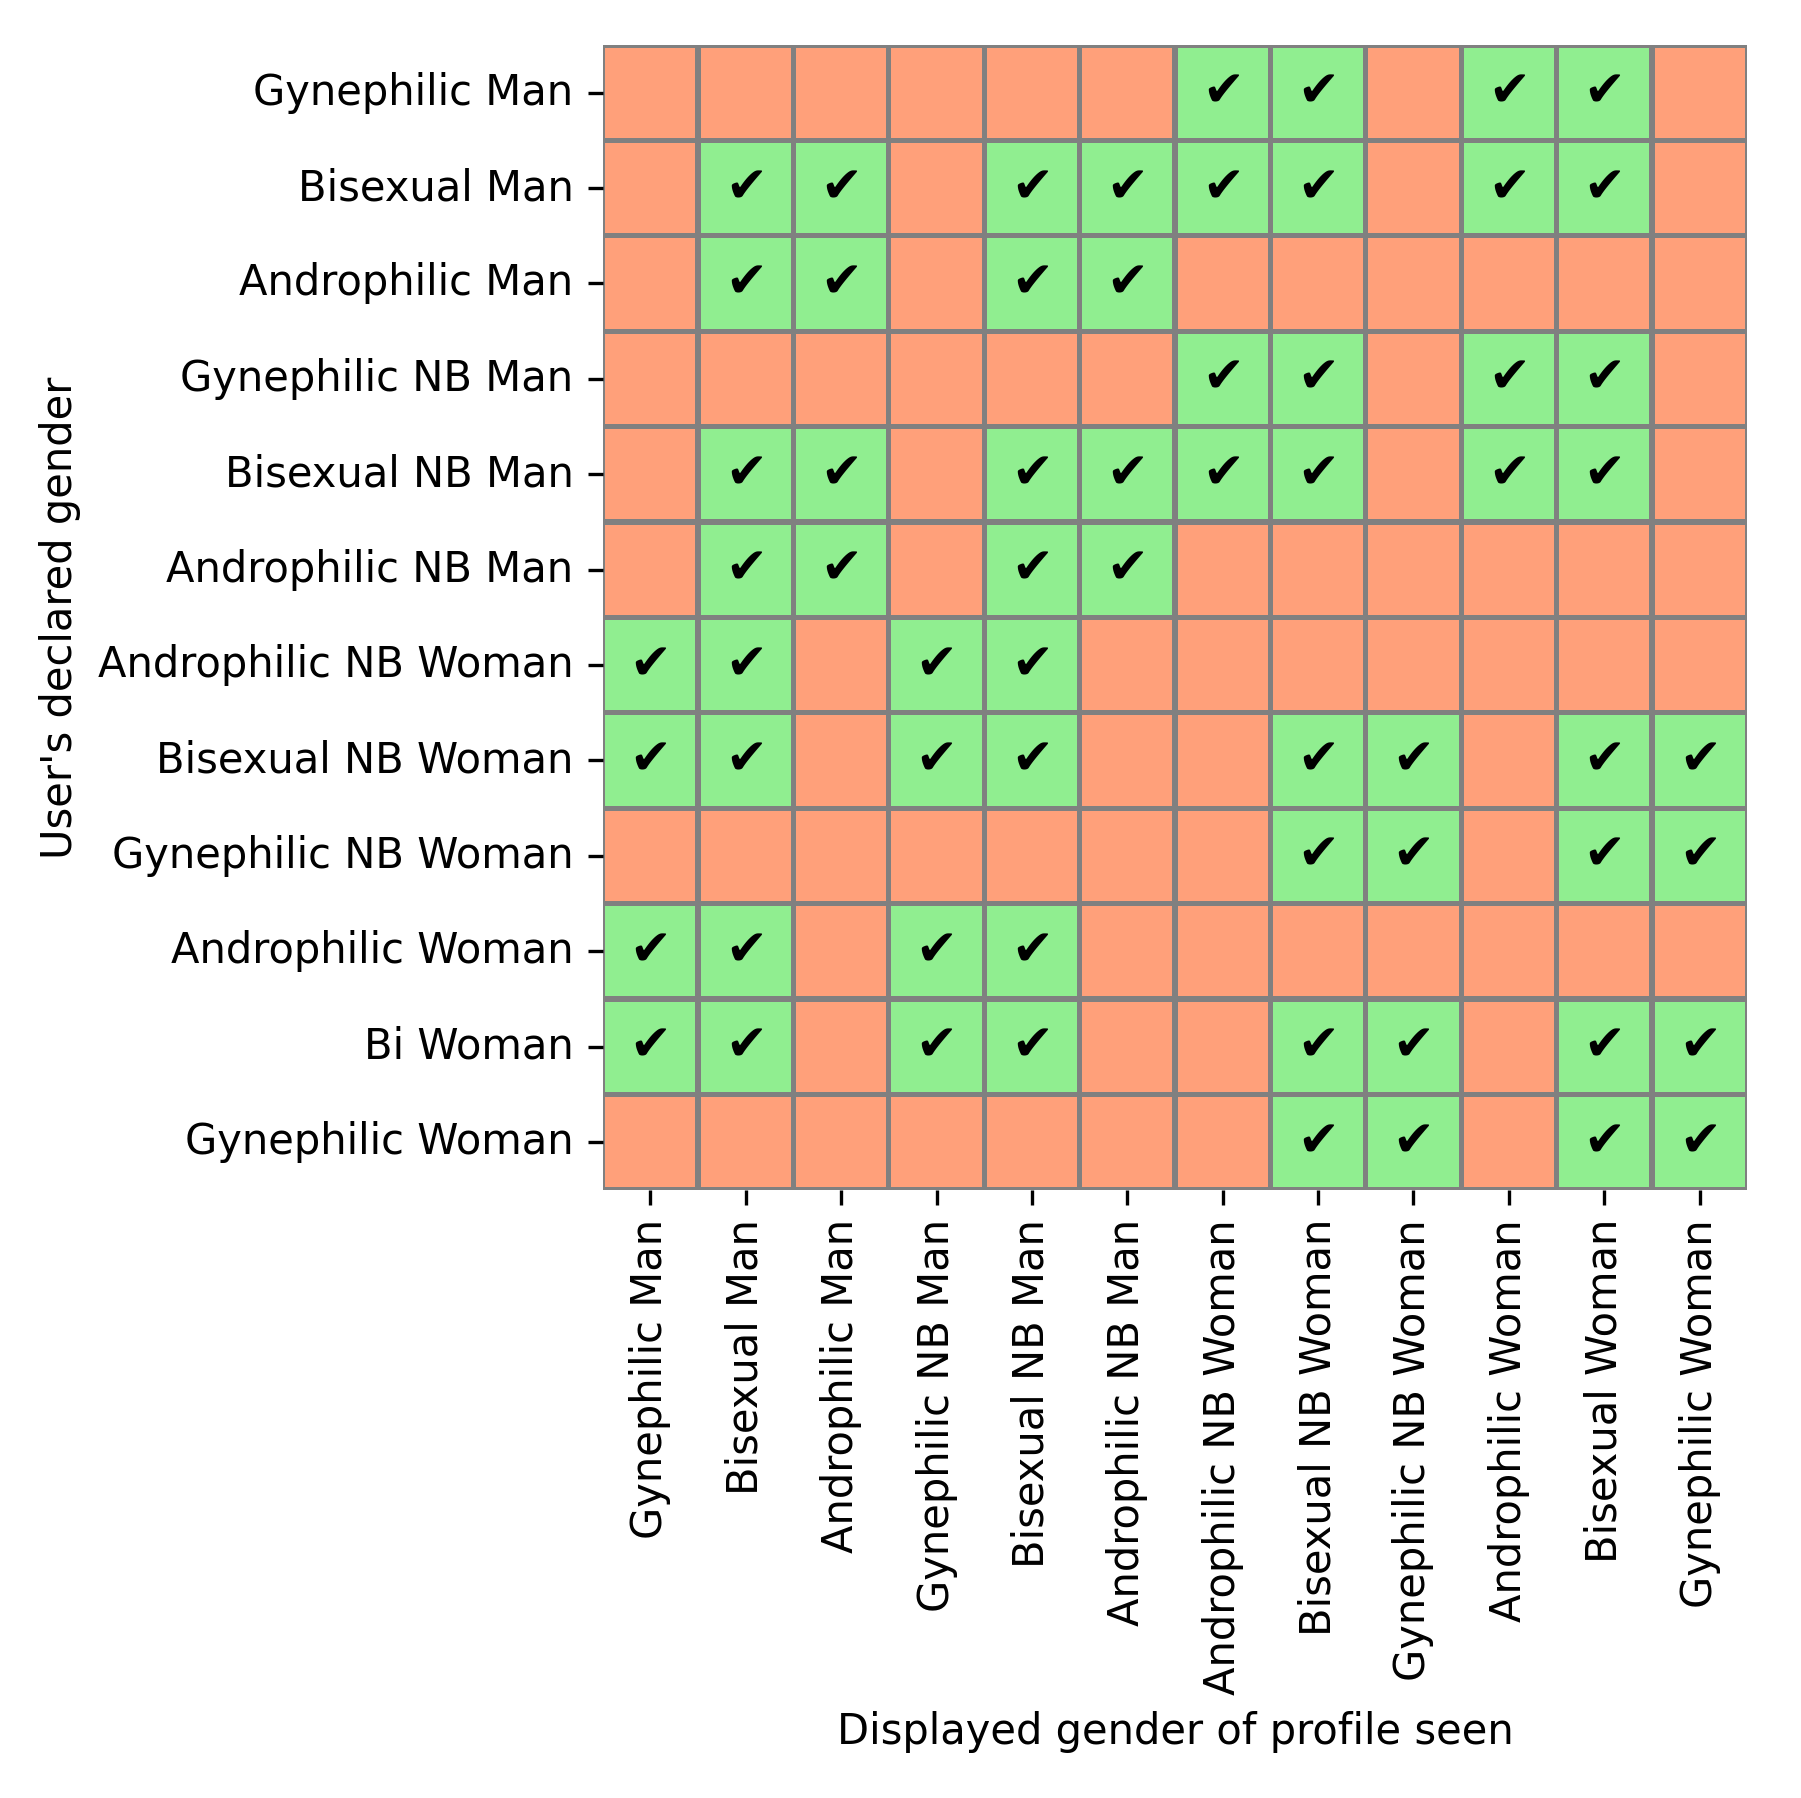
\includegraphics[scale=0.2]{figures/Analysis and Results/gender_matrix.png}
 \caption{Genders-Sexuality Compatibility Grid}
 \label{fig:img3}
\end{figure}

\subsection{Gender Sexuality Comptibility Grid}
The Genders-Sexuality Compatibility Grid Figure \ref{fig:img3} is a atrix const ructed to depict the potential attraction patterns among diverse gender identities and sexual orientations. It systematically represents the interactions between individuals identifying as gynephilic (attracted to women), androphilic (attracted to men), bisexual, across male, non-binary (NB), and female spectrums. Green checkmarks (\checkmark) in the grid signify mutual attraction or compatibility, while red backgrounds indicate incompatibility or lack of attraction.

The development of this grid is grounded in empirical data derived from interviews, and corroborated by analyses of scholarly articles and research papers that explore gender identity and sexual orientation. For instance, studies on childhood gendered behavior and adult sexual attraction patterns provide evidence of the diversity in attraction preferences among androphilic and gynephilic individuals \cite{Petterson_Wrightson_Vasey_2017}.

Research into the sexual attraction of Samoan cisgender and transgender individuals to men and women reveals the intricate cultural expressions of male androphilia, demonstrating the grid's relevance across different cultures \cite{Petterson_Wrightson_Vasey_2017}. The construct of ambiphilia or bisexuality is further substantiated through implicit cognition studies, confirming attraction to both genders \cite{Snowden_Fitton_McKinnon_Gray_2020}.

Moreover, evolutionary perspectives on male androphilia elucidate the shared biological and developmental correlates underlying this sexual orientation, informing the structure of the grid \cite{Vasey_VanderLaan_2014}. These insights confirm that, despite differences in cultural gender roles, sexual attraction follows consistent patterns.

Using this matrix, we were able to systematically track and analyze the distribution and frequency of match recommendations across different gender pairings. This method allowed us to discern patterns or biases in how the algorithm recommends profiles, which is crucial for understanding the extent to which Bumble’s algorithm might perpetuate existing societal biases.

\subsection{Verification of Demographic Parity}
To assess fairness in algorithmic recommendations, we employed the concept of demographic parity. This involves comparing the match recommendations received by binary gender users (men and women) with those received by their non-binary counterparts. When setting your gender as Non-Binary on Bumble, it asks you to fill in which gender categroy you want your profile to show as, i.e., either Man or Woman. So for the purpose of this study, we define the non-binary counterparts as follows:

\begin{itemize}
    \item \textbf{Non-Binary Man:} A profile set up by a participant with Non-Binary as gender, and 'Appear in Searches' as Man.
    \item \textbf{Non-Binary Woman:} A profile set up by a participant with Non-Binary as gender, and 'Appear in Searches' as Woman.
\end{itemize}

These definitions align with the operationalization of gender in our dataset, ensuring that the comparisons we make are grounded in the lived experiences of non-binary individuals using Bumble.

By verifying demographic parity, we aimed to discover whether the algorithm shows a preference for certain genders, thereby disadvantaging others. This analysis involved comparing the rates at which different genders were shown to man vs. non-binary man and woman vs. non-binary woman profiles. It is a crucial step in determining whether the matching algorithm enforces or mitigates gender bias, thereby influencing the inclusivity and fairness of the platform.

\subsection{Statistical Techniques}
The primary statistical technique employed in this analysis was the Chi-squared test of independence. This test was used to examine the relationship between the gender identity of the profile user (man, non-binary man, woman, non-binary woman) and the gender identity of the profiles they were shown by Bumble's matching algorithm. The Chi-squared test is particularly useful for categorical data analysis, as it helps determine whether there is a statistically significant association between two categorical variables.

For this study, the Chi-squared test allowed us to assess the null hypothesis that gender identity of the user does not influence the gender of the profiles shown to them. This hypothesis was tested across different gender pairings within the data, such as man versus non-binary man and woman versus non-binary woman, to identify any disparities in how different genders were treated by the algorithm.

The result of the Chi-squared test yielded a p-value of 0.039, indicating that there are statistically significant differences in the distribution of gender in match recommendations based on the user’s gender identity. This finding suggests that the algorithm may be influencing match recommendations in a way that does not equally represent gender identities, thus potentially contributing to a bias in how users are paired on the platform.

This statistical evidence forms a critical part of the analysis, as it provides a quantitative basis for discussing algorithmic fairness and the representation of gender diversity in Bumble's match recommendations.

\section{Profile Analysis Results}
The results of our analysis highlight significant findings regarding the gender distribution in match recommendations provided by Bumble. The primary attribute analyzed was the gender of profiles recommended to users of different gender identities. We quantified the profiles by gender for each user, normalized these counts against the total number of profiles displayed, and calculated the mean for users of each declared gender. This methodological approach enabled a rigorous evaluation of the distribution of profiles across genders, offering a systematic understanding of how the algorithm mediates match recommendations based on user gender.

\begin{figure}[t!]
 \centering
 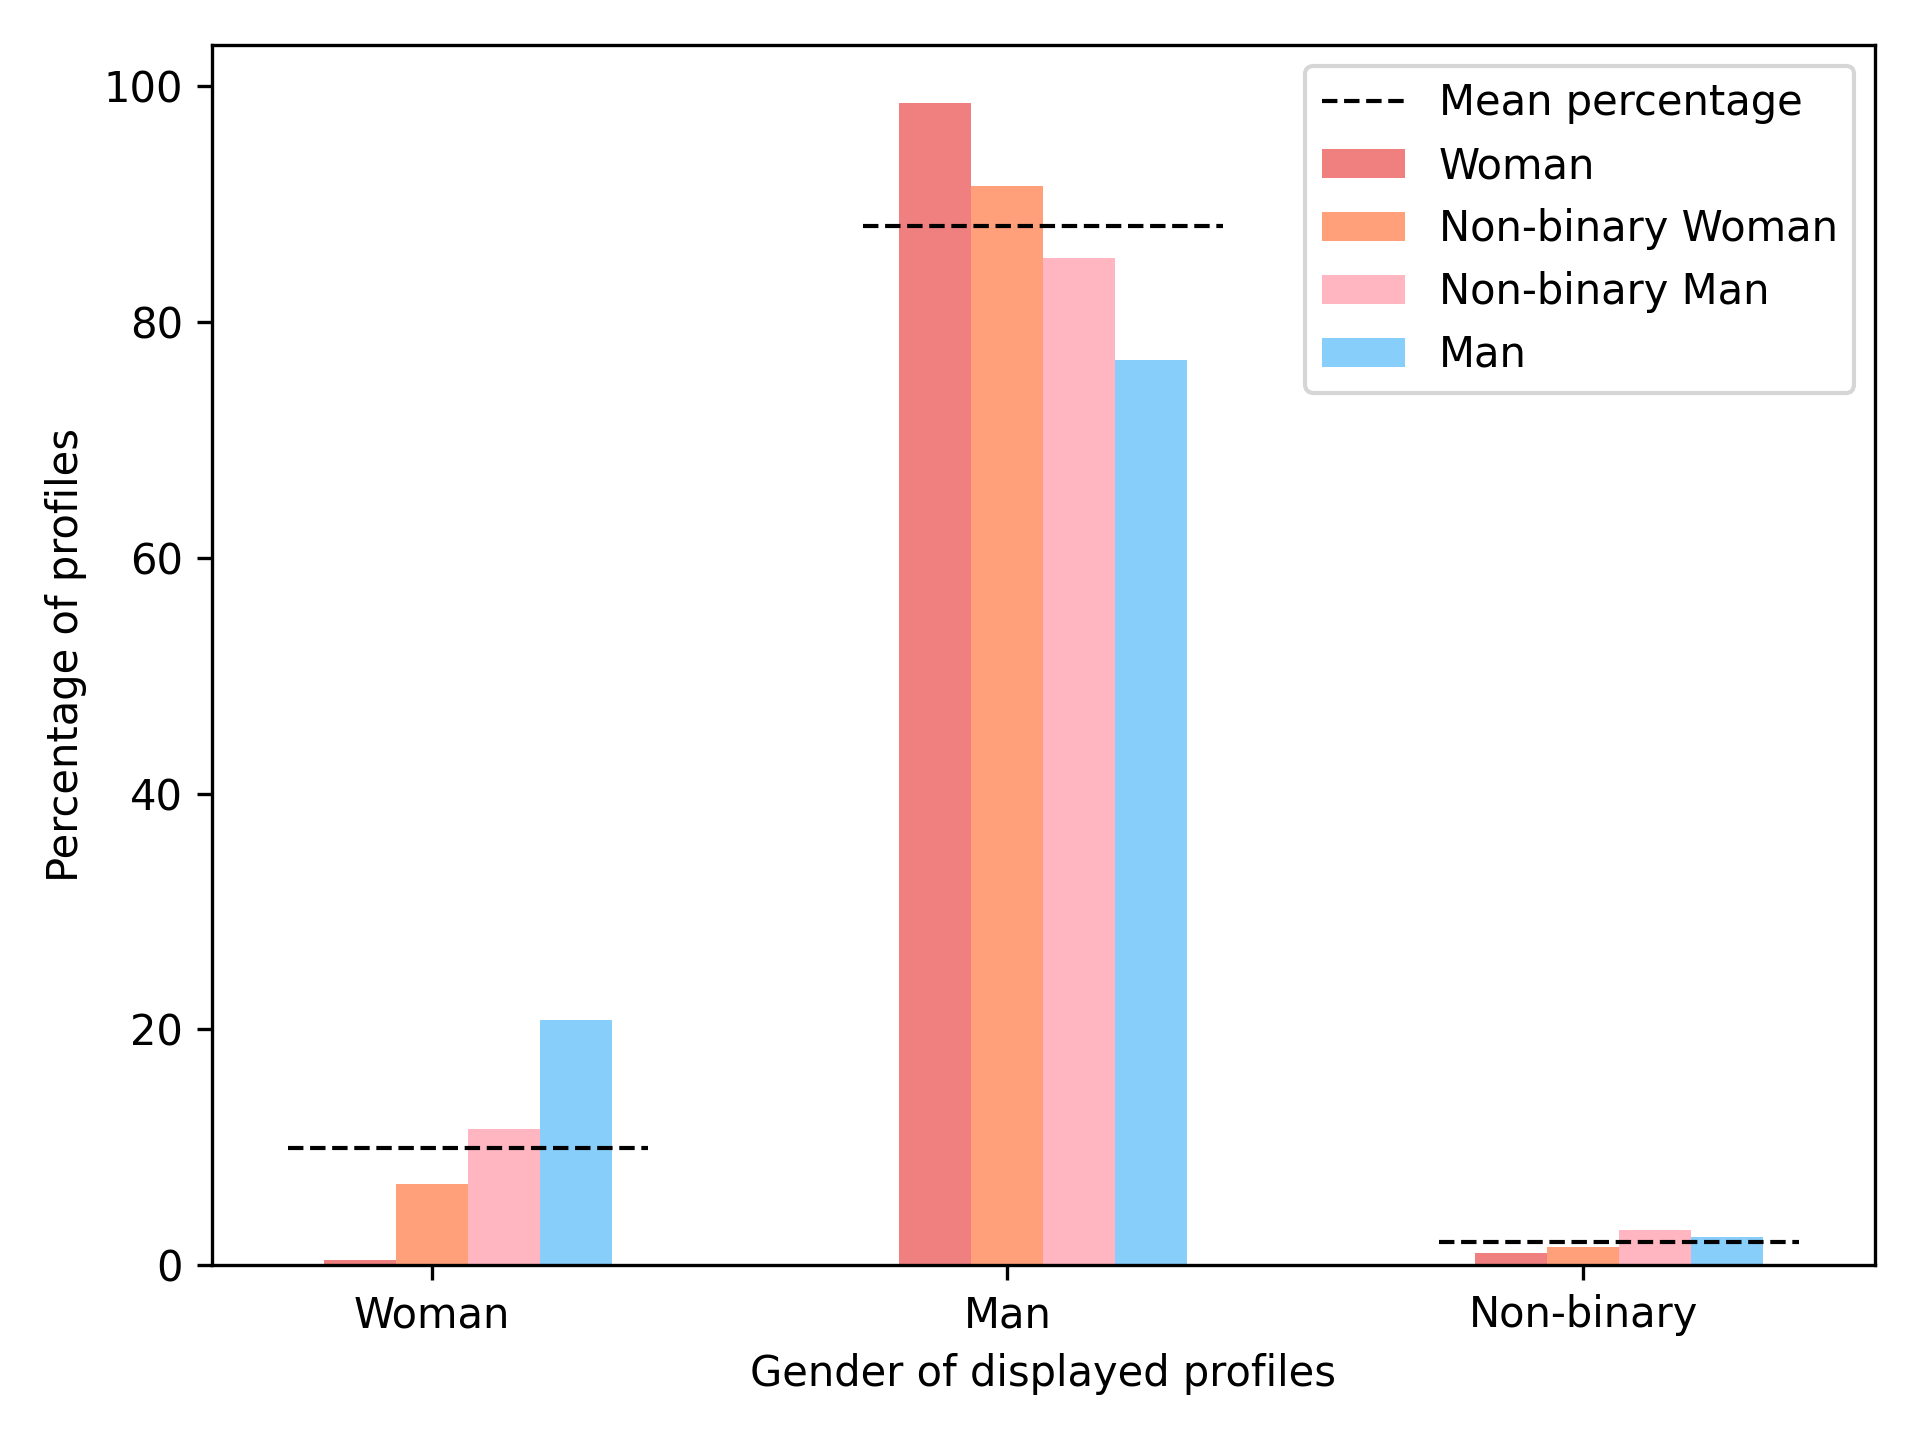
\includegraphics[scale=0.8]{figures/Analysis and Results/gender_percentage.png}
 \caption{Percentage of Genders displayed in our Profiles}
 \label{fig:img4}
\end{figure}

Our analysis revealed discernible skews in the gender distribution of match recommendations. Notably, for our male profiles, the number of female profiles displayed was 9.1\% higher compared to their non-binary male counterparts. Conversely, female profiles experienced a 6.8\% higher exposure to male profiles than did their non-binary female counterparts. These disparities suggest a potential bias in the algorithm's recommendation system, where the gender identity of the user appears to influence the gender composition of the profiles shown. This finding is significant as it suggests that Bumble’s algorithm may not treat gender identity neutrally but rather modulates match visibility in a way that could disadvantage non-binary users.

Another significant trend observed in our analysis concerns the skewed distribution between the number of men and women displayed to users. Generally, the proportion of men shown to users is substantially higher. This trend reflects the overall gender ratio among Bumble users, as derived from our dataset, where men constitute 88.12\% of profiles, women make up 9.92\%, and non-binary individuals account for 1.96\%.

This imbalance in gender representation is even more pronounced when comparing the gender ratios of the profiles shown with the gender of the participants themselves. Specifically, our findings show that men are disproportionately shown to women users compared to how often women are shown to men users. This indicates a potential bias in the algorithm’s process of generating match recommendations, which tends to favor the display of male profiles over female or non-binary profiles.

\section{Interviews Analysis}
The qualitative insights derived from interviews conducted with Bumble users, particularly those who identify as bisexual, offer a detailed look into the lived experiences and challenges faced on the dating platform. These interviews shed light on the nuanced ways in which the application’s algorithms impact user experiences, particularly in terms of gender representation and the accuracy of match recommendations. The firsthand accounts reveal not only algorithmic shortcomings but also provide critical user perspectives on the platform's operational dynamics.

\subsection{Key Themes from the Interviews}
\begin{itemize}
    \item \textbf{Discrepancies in Gender Representation:} Interviewees frequently pointed out a significant skew in gender representation, especially noting an overrepresentation of male profiles despite their preferences set for females. This discrepancy is crucial as it reflects a misalignment between user settings and profile recommendations, with one user expressing, "I'm shown more men than women even when I don’t have everyone (filter) on... it's like an epidemic just men marking their profile as women whose preference is women" (Subject A). Another user highlighted, "It's mostly men being shown - it probably is mostly men because like there's a lot of men on profiles yes but also a lot of men were marked as women are probably shown but because you have everyone turn on you don't notice it" (Subject A), and "I just see a lot of men" (Subject C) underscoring the challenges posed by gender misrepresentation.
    \item \textbf{Algorithmic Limitations and Misclassifications:} The issue of men misrepresenting their gender to appear in searches intended for women was a significant concern, particularly affecting lesbian and bisexual women. This misclassification leads to frustration and mistrust in the platform's ability to cater effectively to user preferences, as evidenced by comments from the interviews: "I'll show you something yeah but it's like an epidemic just men marking their profile as women whose preference is women" (Subject A).
    \item \textbf{Impact on User Experience and Preferences:} The frustrations stemming from discrepancies in gender representation and algorithmic misclassification directly diminish user experience and satisfaction. As one user bluntly put it, "I have everyone right now, I don't enjoy using Bumble" (Subject A).
    \item \textbf{Safety and Inclusivity Concerns:} Safety issues emerged as a recurrent theme, with users feeling unsafe due to the misrepresentation of profiles and the absence of robust filters to mitigate such experiences. This is captured in remarks such as, "Also like it feels a little unsafe to just meet a random man from a dating profile as opposed to like uh of a woman" (Subject A), and "I used to see that ('Potential Match Missed' message) at time and that would be after I swiped left on (let's say) a 30-40 year old man and that was creepy for me" (Subject B) and the need for platform improvements: "Fixing the men marking themselves as women thing definitely would be like a very major thing because it's literally like taking you off the app" (Interview 5).
    \item \textbf{Potential for Algorithmic Improvement:} Users suggested several improvements to enhance the algorithm, such as better filtering options and the capability to have separate feeds for different genders, which could significantly enhance user experience. These suggestions are encapsulated in statements like, "If it like um showed you not like equally but like based on how much you have swiped in the past on women versus men that would probably be a good like balance" (Subject A), and "I think they should have different recommendation algorithms for men and women" (Subject A), indicating a pathway towards more personalized and effective matching processes.
\end{itemize}  

\section{Integration of Quantitative and Qualitative Insights}
The quantitative analysis of profile distributions and the qualitative insights gained from user interviews in this study complement each other, providing a holistic understanding of the gender biases present in Bumble's matchmaking algorithms.

The quantitative analysis involved systematically counting and normalizing the profiles by gender shown to each participant. This data provided a clear, objective measure of how gender influences the profiles that users are shown. By quantifying these distributions, we established a baseline understanding of the gender dynamics within the app. The statistical significance of these findings, evidenced by disparities in gender representation (men being predominantly shown to women and vice versa), underscores potential biases in the algorithm's recommendation system.

On the other hand, the interviews offered nuanced, subjective insights that qualitative data alone could not capture. Participants shared their personal experiences and perceptions regarding the diversity and inclusiveness of the profiles they encountered. These discussions revealed the practical impact of the observed quantitative disparities on user experience. For instance, several female and non-binary participants noted a sense of frustration or exclusion due to the overwhelming number of male profiles, which aligned with the quantitative data showing a higher percentage of male profiles in their match recommendations.

Together, these methods paint a comprehensive picture of the algorithm's behavior and its effects on users. The quantitative data highlights systemic issues and patterns that require attention, while the qualitative insights provide context and depth, illustrating how these patterns affect real people's interactions on the platform. This dual approach not only strengthens the validity of the findings by corroborating quantitative data with real-world experiences but also enriches the discussion on how to improve algorithmic fairness and inclusivity in digital dating spaces.

\section{}

%--------------------------------------------------------

\chapter{Discussions}
\label{ch:conc}
\section{Summary of the Findings}
The study we've conducted revealed significant biases in how the algorithm recommends matches, with pronounced disparities affecting users of non-binary genders. These findings underscore a broader issue of algorithmic bias within digital dating environments, reflecting societal norms and potentially reinforcing gender stereotypes.

The study found that Bumble's algorithm tends to replicate existing societal biases, which are then manifested in the match recommendations provided to users. Non-binary users, in particular, experienced a marked reduction in the visibility and accessibility of suitable matches, suggesting that the algorithm is optimized for binary gender preferences and fails to accommodate the diversity of gender identities effectively. This aligns with broader findings in the field that suggest algorithms, while ostensibly neutral, often perpetuate the biases present in their training data or design logic \cite{davidson-etal-2019-racial,Selbst_Boyd_Friedler_Venkatasubramanian_Vertesi_2019}.

The disparities in match recommendations not only influence the user experience but can also impact users' perceptions of the app's inclusivity. Non-binary users reported feeling marginalized by the platform, which could deter continued use or engagement. This finding is particularly concerning given the increasing reliance on digital platforms for social interactions and the potential of these platforms to shape social norms \cite{MacLeod_McArthur_2019}.

The empirical evidence from the study suggests a discrepancy between theoretical expectations of algorithm neutrality and the actual performance of these systems. Despite Bumble's claims of promoting a progressive and inclusive dating environment, the algorithmic practices observed align more closely with traditional gender norms, thus limiting the platform's potential to foster genuinely inclusive interactions. These findings resonate with the concerns raised by researchers regarding the ethical implications of algorithmic decision-making in social platforms \cite{Hutson_Taft_Barocas_Levy_2018}.

The replication of biases has broader implications for the role of technology in society. As algorithms increasingly influence various aspects of social life, the biases they carry can have far-reaching effects on social equity and personal identity. This underscores the need for more rigorous approaches to algorithm design and a stronger regulatory framework to ensure fairness and inclusivity in digital interactions \cite{Lambrecht_Tucker_2019}.

\section{Algorithmic Bias and Societal Impact}
We explore now the relationship between algorithmic bias in Bumble's match recommendations and its broader societal impacts. We delve into how these biases influence not only individual user experiences but also perpetuate existing social inequalities, shaping the digital and social landscape.

The research highlights that Bumble's algorithm, though designed to facilitate connections based on user preferences, inadvertently prioritizes profiles that conform to binary gender norms. This bias is evident in the algorithm's tendency to present a disproportionate number of opposite-gender matches to users, irrespective of their stated preferences for non-binary identities. Such a design reflects and perpetuates heteronormative assumptions prevalent in society, limiting the visibility of non-binary and gender-diverse users within the platform. This finding aligns with prior research indicating that many digital platforms inherently encode societal biases, whether through the data they utilize or the design choices made by developers \cite{Noble_2018, Benjamin_2019}.

The implications of these biases extend beyond the digital realm into broader social contexts. By reinforcing binary gender norms, Bumble's algorithm not only affects individual user experiences but also contributes to a culture that marginalizes non-binary identities. This can perpetuate a cycle of exclusion and discrimination that affects societal perceptions of gender and sexuality. The influence of such algorithms on social norms is profound, as they have the power to shape interactions and relationships in significant ways \cite{Eubanks_2018}.

Drawing comparisons with other technologies, the study situates Bumble within a broader ecosystem of algorithmic decision-making platforms, such as social media and employment algorithms, which have been shown to exhibit similar biases. Like Bumble, these platforms often reflect and amplify existing social inequalities, suggesting a pervasive issue across different sectors. The comparative analysis underscores the need for comprehensive approaches to address algorithmic biases across all digital platforms \cite{ONeil_2016}.

To mitigate these issues, the thesis proposes several interventions:
\begin{itemize}
    \item \textbf{Enhancing Algorithmic Transparency:} Encouraging companies like Bumble to disclose more about how their algorithms operate can foster greater accountability and allow for the identification and correction of biases.
    \item \textbf{Inclusive Design Practices:} Designing algorithms with inclusivity as a foundational principle can help ensure that all user identities are equally represented and valued. This includes incorporating diverse datasets and perspectives in the development process to minimize bias \cite{Costanza-Chock_2020}.
    \item \textbf{Regular Auditing and Updates:} Implementing regular audits of algorithmic processes to ensure they remain fair and effective over time, adapting to changes in societal norms and technological advancements.
\end{itemize}

The broader societal impact of these platforms varies by their approach to inclusivity. Platforms that have made a deliberate effort to include diverse identities tend to foster a more welcoming environment, potentially influencing societal attitudes towards diverse gender and sexual identities. This aspect is crucial because the representation and treatment of non-binary and transgender individuals on these platforms can reflect and influence societal norms. By promoting inclusivity and diversity, digital platforms can contribute positively to social change and equity \cite{Kalra_Gupta_Varghese_Rangaswamy_2023}.

\section{Methodological Reflections}
The study employed a mixed-methods approach, combining quantitative data analysis with qualitative interviews to provide a holistic view of the algorithmic biases present in Bumble's match recommendations. This approach allowed for a detailed examination of both the numerical trends in user interactions and the personal experiences and perceptions of users, particularly those from non-binary and gender-diverse communities \cite{Kalra_Gupta_Varghese_Rangaswamy_2023}.

One of the key strengths of this approach is its ability to cross-validate findings across different data sources and methodologies:

\begin{itemize}
    \item \textbf{Quantitative Analysis:} Provided robust data on user behavior and match patterns, which helped identify systemic biases in the algorithm. 
    \item \textbf{Qualitative Interviews:} Offered deep insights into the subjective experiences of users, enriching the understanding of the data's practical implications on real-life user experiences \cite{Kalra_Gupta_Varghese_Rangaswamy_2023}.
\end{itemize}
This mixed-methods approach is particularly effective in exploring complex social phenomena like algorithmic bias, as it captures both the breadth and depth of the issue \cite{Creswell_2009}

Despite its strengths, the study faced several limitations:

\begin{itemize}
    \item \textbf{Sample Size and Diversity:} While efforts were made to include a diverse range of participants, the relatively small sample size and the focus primarily on one geographical location may limit the generalizability of the findings to other settings or populations.
    \item \textbf{Algorithmic Opacity:} The proprietary nature of Bumble’s algorithm limited the ability to directly observe how decisions are made within the system, necessitating reliance on external manifestations of its behavior, such as user-reported experiences and match patterns 
\end{itemize}

\section{Implications of Design and Policy}
The study underscores the necessity of incorporating inclusivity at the earliest stages of algorithm design. Dating apps should consider diverse gender identities and sexual orientations from the outset, ensuring that the algorithm is capable of understanding and adapting to a wide range of user preferences. This could involve:

\begin{itemize}
    \item Designing user interfaces that explicitly accommodate a variety of gender presentations, going beyond the traditional binary options.
    \item Adjusting match algorithms to equally prioritize non-binary and gender-nonconforming users, rather than merely adapting binary algorithms that may not adequately address their needs \cite{Kalra_Gupta_Varghese_Rangaswamy_2023}
\end{itemize}

To ensure that algorithms remain relevant and non-discriminatory over time, it is crucial to integrate regular feedback mechanisms into the app. User feedback can provide real-time insights into how well the algorithm meets diverse needs and highlight areas for improvement. This approach can facilitate continuous learning and adaptation, ensuring that the services evolve in line with user expectations and societal changes \cite{Kalra_Gupta_Varghese_Rangaswamy_2023}.

Transparency about how algorithms make match recommendations can build trust and allow users to make informed choices about their interactions on the platform. By disclosing the factors that influence match suggestions, apps can empower users to better understand and potentially challenge decisions made by the algorithm. This transparency is also crucial for regulatory oversight and accountability \cite{PASQUALE_2015}.

Policymakers should consider developing comprehensive guidelines that address algorithmic discrimination, specifically in the context of digital platforms like dating apps. These guidelines could mandate:

\begin{itemize}
    \item Regular audits of algorithms to assess bias.
    \item The implementation of corrective measures when discriminatory practices are identified.
    \item Reporting requirements to monitor compliance and effectiveness of anti-bias measures \cite{Eubanks_2018}
\end{itemize}

Governments and regulatory bodies could provide incentives for the development of ethical AI technologies. This could include funding for research into inclusive algorithm design, grants for startups committed to ethical practices, and awards for innovations that significantly reduce bias in digital platforms. Such policies would not only foster innovation but also ensure that it proceeds along ethically sound lines \cite{Crawford_Calo_2016}

Legislation may be required to enforce transparency and accountability in digital platforms' use of algorithms. This could involve:

\begin{itemize}
    \item Laws mandating that companies disclose the logic, importance, and consequences of their algorithms.
    \item Regulations ensuring that users can opt-out of certain algorithmic decisions or appeal against them if they feel discriminated against.
    \item Frameworks for users to understand how their data is being used and to control it \cite{Kaminsiki_2019}.
\end{itemize}

\section{Future Research Directions}
This thesis has laid foundational groundwork on the impact of algorithmic biases in dating apps like Bumble, particularly regarding gender disparities. To advance this critical area of study, several avenues for future research can be explored, leveraging interdisciplinary approaches that blend technology, sociology, and behavioral science. These directions not only promise to deepen the understanding of existing problems but also to innovate in ways that might mitigate biases more effectively.

Future research could focus on conducting comprehensive algorithmic audits across multiple dating platforms. These audits would assess how different algorithms perform in terms of equity and fairness across diverse demographic groups. By comparing platforms with different operational models and user bases, researchers can identify best practices and common pitfalls. Incorporating methodologies from data science and algorithmic fairness can provide quantitative rigor, while insights from sociology help contextualize the results within broader social structures.

Investigating how user behavior and platform algorithms evolve over time can provide valuable insights into the dynamic interplay between user interaction and algorithmic recommendation systems. Longitudinal studies could track changes in user behavior in response to modifications in the app's algorithms, interface, or policy changes. Such studies would benefit from a combination of behavioral science methods to gauge changes in user perception and technology studies to understand algorithmic adjustments over time.

While quantitative data is invaluable, qualitative research offers depth and nuance that numbers alone cannot provide. Future studies should include in-depth interviews, focus groups, and ethnographic research with users from a wide array of gender identities and sexual orientations. Sociology and anthropology provide robust frameworks for understanding cultural and social dynamics, which are crucial for interpreting how individuals experience and are impacted by algorithmic decisions in their social and personal lives.

Given the global reach of dating apps, comparing how algorithms function in different cultural contexts can uncover unique challenges and opportunities for fostering inclusivity. Research could examine how cultural variables influence algorithmic bias and user experience in different regions. This approach would benefit from a combination of cultural studies to understand societal norms and expectations, and comparative studies in technology policy to see how different regulatory environments impact algorithm design and function.

Encouraging the development of new algorithmic models that prioritize inclusivity and fairness from the ground up is another crucial research direction. This could involve collaborations between computer scientists, ethicists, and sociologists to design algorithms that not only respond to user behaviors but also proactively mitigate potential biases. Behavioral science can inform the design of these systems by providing insights into human behavior that can predict how changes in algorithms might influence user interaction.

Finally, exploring the ethical and policy implications of algorithmic decision-making in dating apps is essential. This research could inform policymakers and stakeholders about the necessary regulations to ensure fairness and equity in digital spaces. It would benefit from interdisciplinary collaboration involving legal studies, ethics, technology policy, and social justice advocacy.

By pursuing these directions, future research can contribute significantly to creating more equitable and inclusive digital environments, ensuring that technology serves the diverse needs of all its users.

\section{Conclusion}
In this thesis, we have examined the intricate ways in which Bumble's algorithm, designed to facilitate romantic connections, inadvertently perpetuates existing societal biases. These biases, deeply embedded in the datasets from which the algorithm learns, reflect long-standing human and cultural prejudices that significantly impact users with diverse gender identities. As Raghavan et al. \cite{Raghavan_Barocas_Kleinberg_Levy_2019} highlight, these algorithmic biases not only mirror but can also amplify the biases present within their training data, perpetuating a cycle of discrimination and exclusion within the digital dating space.

The study has demonstrated that Bumble's algorithm does not operate in a vacuum but is influenced by the socio-cultural context of its data. This means that biases inherent in societal structures and historical data are likely to be reproduced and even intensified by algorithmic decisions. This reproduction of biases affects how individuals with diverse gender identities experience the platform, often marginalizing them in favor of more mainstream user profiles. This finding is consistent with the broader discourse on algorithmic fairness, which suggests that without careful intervention, algorithms tend to favor the status quo, thereby reinforcing existing inequalities \cite{heidivellastarr_2022}

The ethical implications of these findings are significant. As developers and operators of such platforms, there is a moral responsibility to ensure that the systems created do not harm users or perpetuate harm. This moral agency is derived from the choices made during the design and operation of these algorithms \cite{Mittelstadt_2016}. Ensuring that these choices are conscious of inclusivity and fairness is crucial, particularly in a country as diverse as India.

To address these challenges, it is essential to adopt more inclusive design practices. This includes re-evaluating the datasets used for training algorithms to ensure they reflect a broader spectrum of the population and continuously updating these data sets to adapt to changing social norms. Additionally, increasing transparency about how algorithms operate and make decisions can help build trust and accountability, allowing users to understand and potentially challenge biases they encounter \cite{Linden_2020}.

Our study addresses several critical gaps in prior research by employing a uniquely integrated methodological approach that combines quantitative data analysis with qualitative interviews, enabling a deeper understanding of the nuances of gender biases within online dating applications. Unlike many studies that predominantly focus on binary gender perspectives, our research extends to non-binary user experiences, an area that remains significantly under-explored in the context of Indian digital dating landscapes. This methodology not only highlights discrepancies in algorithmic match recommendations but also captures the subjective realities of users, offering insights into how these biases affect individual self-perception and interpersonal dynamics. Moreover, profiling users through online platforms presents inherent challenges, such as ensuring the authenticity of user-reported data and navigating the ethical implications of digital surveillance. Our study mitigates these challenges by adhering to strict ethical guidelines and employing robust data validation techniques, thus ensuring the reliability and credibility of our findings. This comprehensive approach not only fills existing research voids but also contributes to the broader discourse on algorithmic fairness and the need for inclusivity in technological design.

In conclusion, while dating apps like Bumble offer the potential for fostering new social connections, they also pose significant risks of perpetuating and amplifying social biases. By understanding and addressing these risks, developers can not only improve user experiences but also contribute to the broader societal goal of equality and inclusion. Moving forward, it is imperative that the digital arenas we create are as inclusive and equitable as the future we aspire to achieve.


%--------------------------------------------------------
\bibliographystyle{IEEEtran}
\bibliography{IEEEabrv,cite.bib}{}

% %--------------------------------------------------------
% % 'Publication 1'
% \chapter*{Publications}
% \chapter*{Publication 1}
% \addtocontents{toc}{\protect{\addvspace{3.0ex plus 1pt}}}
% \addcontentsline{toc}{chapter}{\protect{Publication 1}}
% \input{sections/paper1.tex}
% \includepdf[pages={-}]{papers/paper1.pdf}
% %
% %--------------------------------------------------------
% % 'Publication 2'
% \chapter*{Publication 2}
% \addtocontents{toc}{\protect{\addvspace{3.0ex plus 1pt}}}
% \addcontentsline{toc}{chapter}{\protect{Publication 2}}
% \input{sections/paper2.tex}
% \includepdf[pages={-}]{papers/paper2.pdf}

\end{document}
